\section{W-mass}
\label{sec:w-mass}
With the finished calibration, the mass of the W-boson can now be measured. This is done using a the Jacobi peak of the electron transverse momentum distribution.
In order to determine the W-mass, we use a data set of actual ATLAS data containing $W \rightarrow e\nu$ events,
as well as several simulated data sets also containing $W \rightarrow e\nu$ events. 
There is also a $Z^0 \rightarrow e^+e^-$ data set to check the validity of the previous calibration.
Finally there are data sets for QCD- and non-QCD background events.

\subsection{Electron Calibration Verification}
    \label{sec:calibration_verification}
    First the previous calibration of the electron energy is verified by examining the $Z^0 \rightarrow e^+e^-$ data set.
    This is done for regions of the detector as well as for different kinematic regions. The different bins of the detector as well as the different kinematic regions
    that were chosen and the resulting $Z^0$ masses are listed in table \ref{tab:z-masses}. The fits to the $m_{ee}$ spectrum can be seen in figure \ref{fig:z-mass_check1} and \ref{fig:z-mass_check2}.

    \begin{figure}
        \begin{subfigure}{0.5\textwidth}
            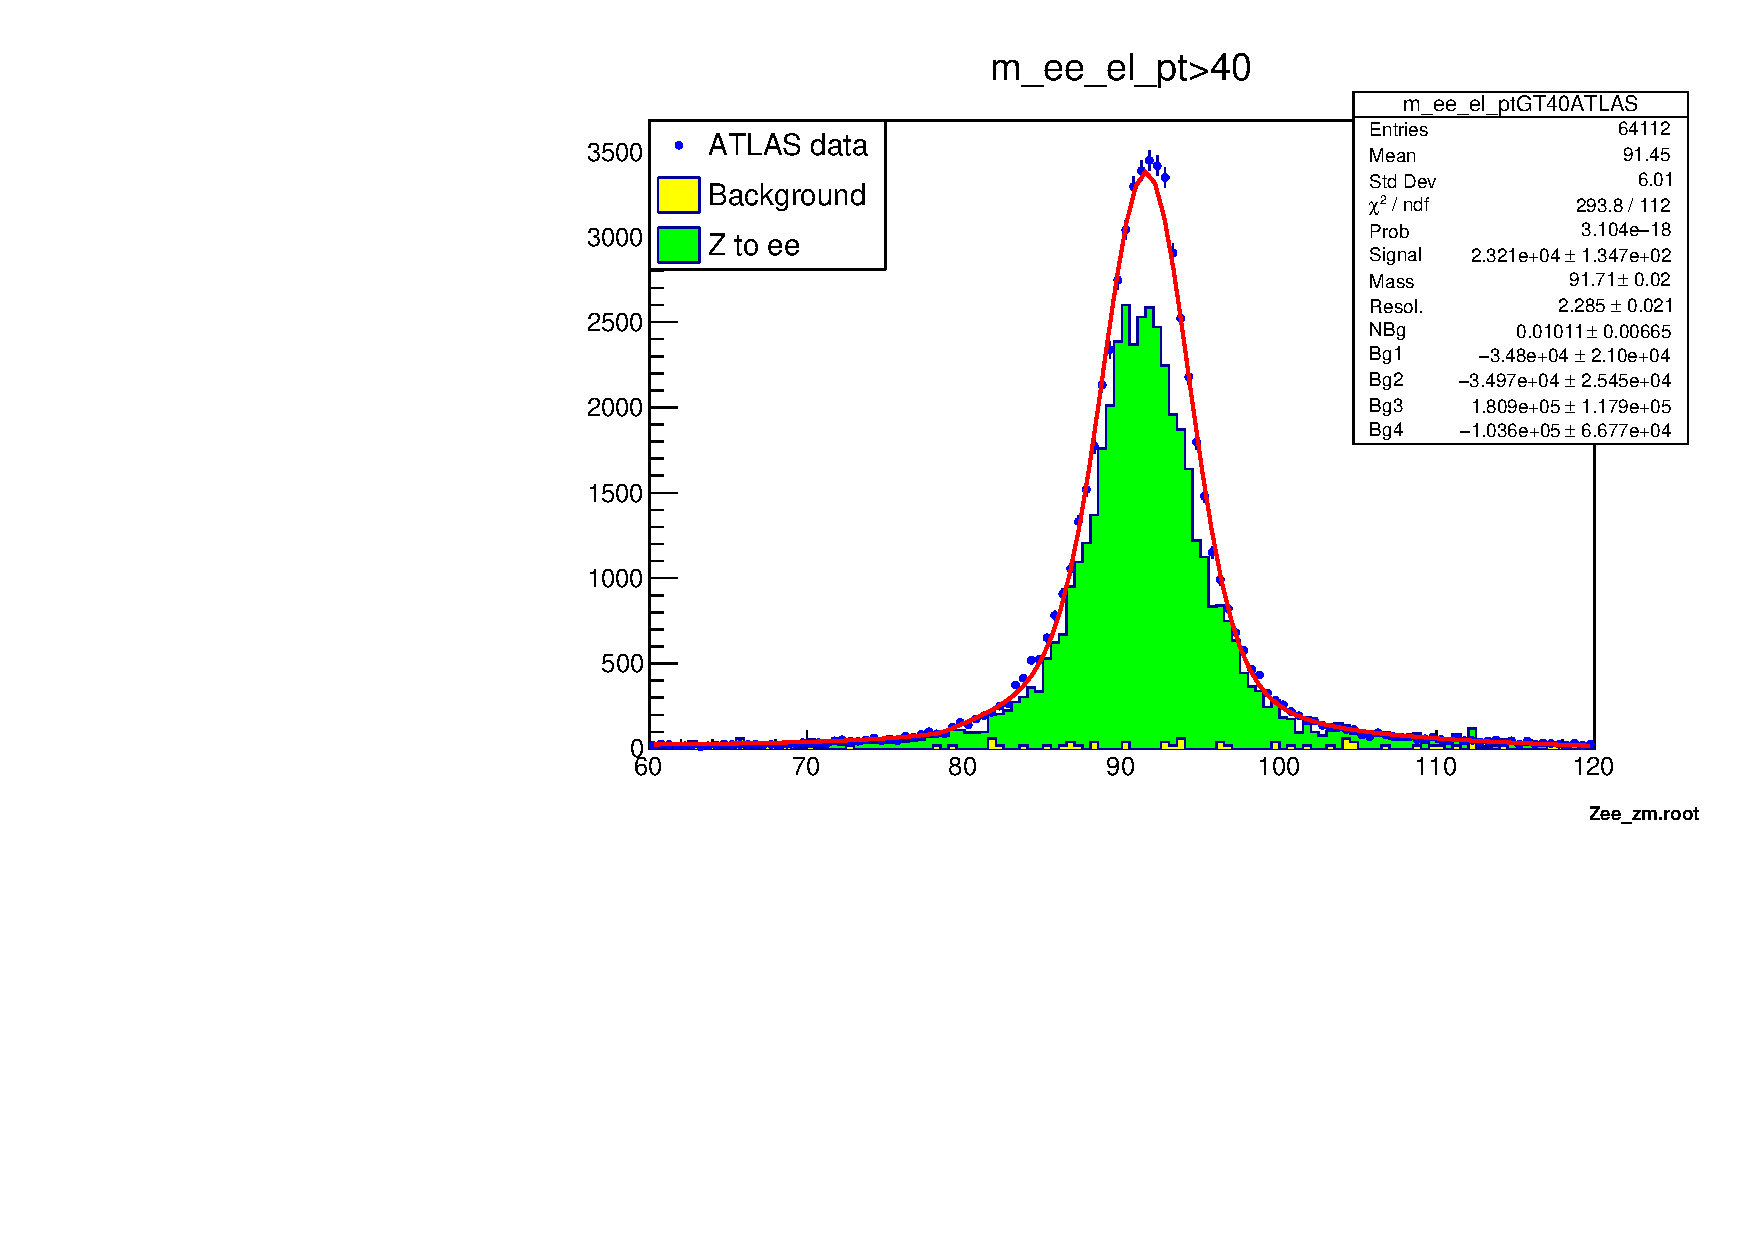
\includegraphics[width=\textwidth]{../W_mass/Z_mass_check_el_pt-cut.pdf}
            \subcaption{Fit to the $Z^0 \rightarrow e^+e^-$ canditates for $p_{T,e^{\pm}} > 40$\,GeV.}
        \end{subfigure}
        \begin{subfigure}{0.5\textwidth}
            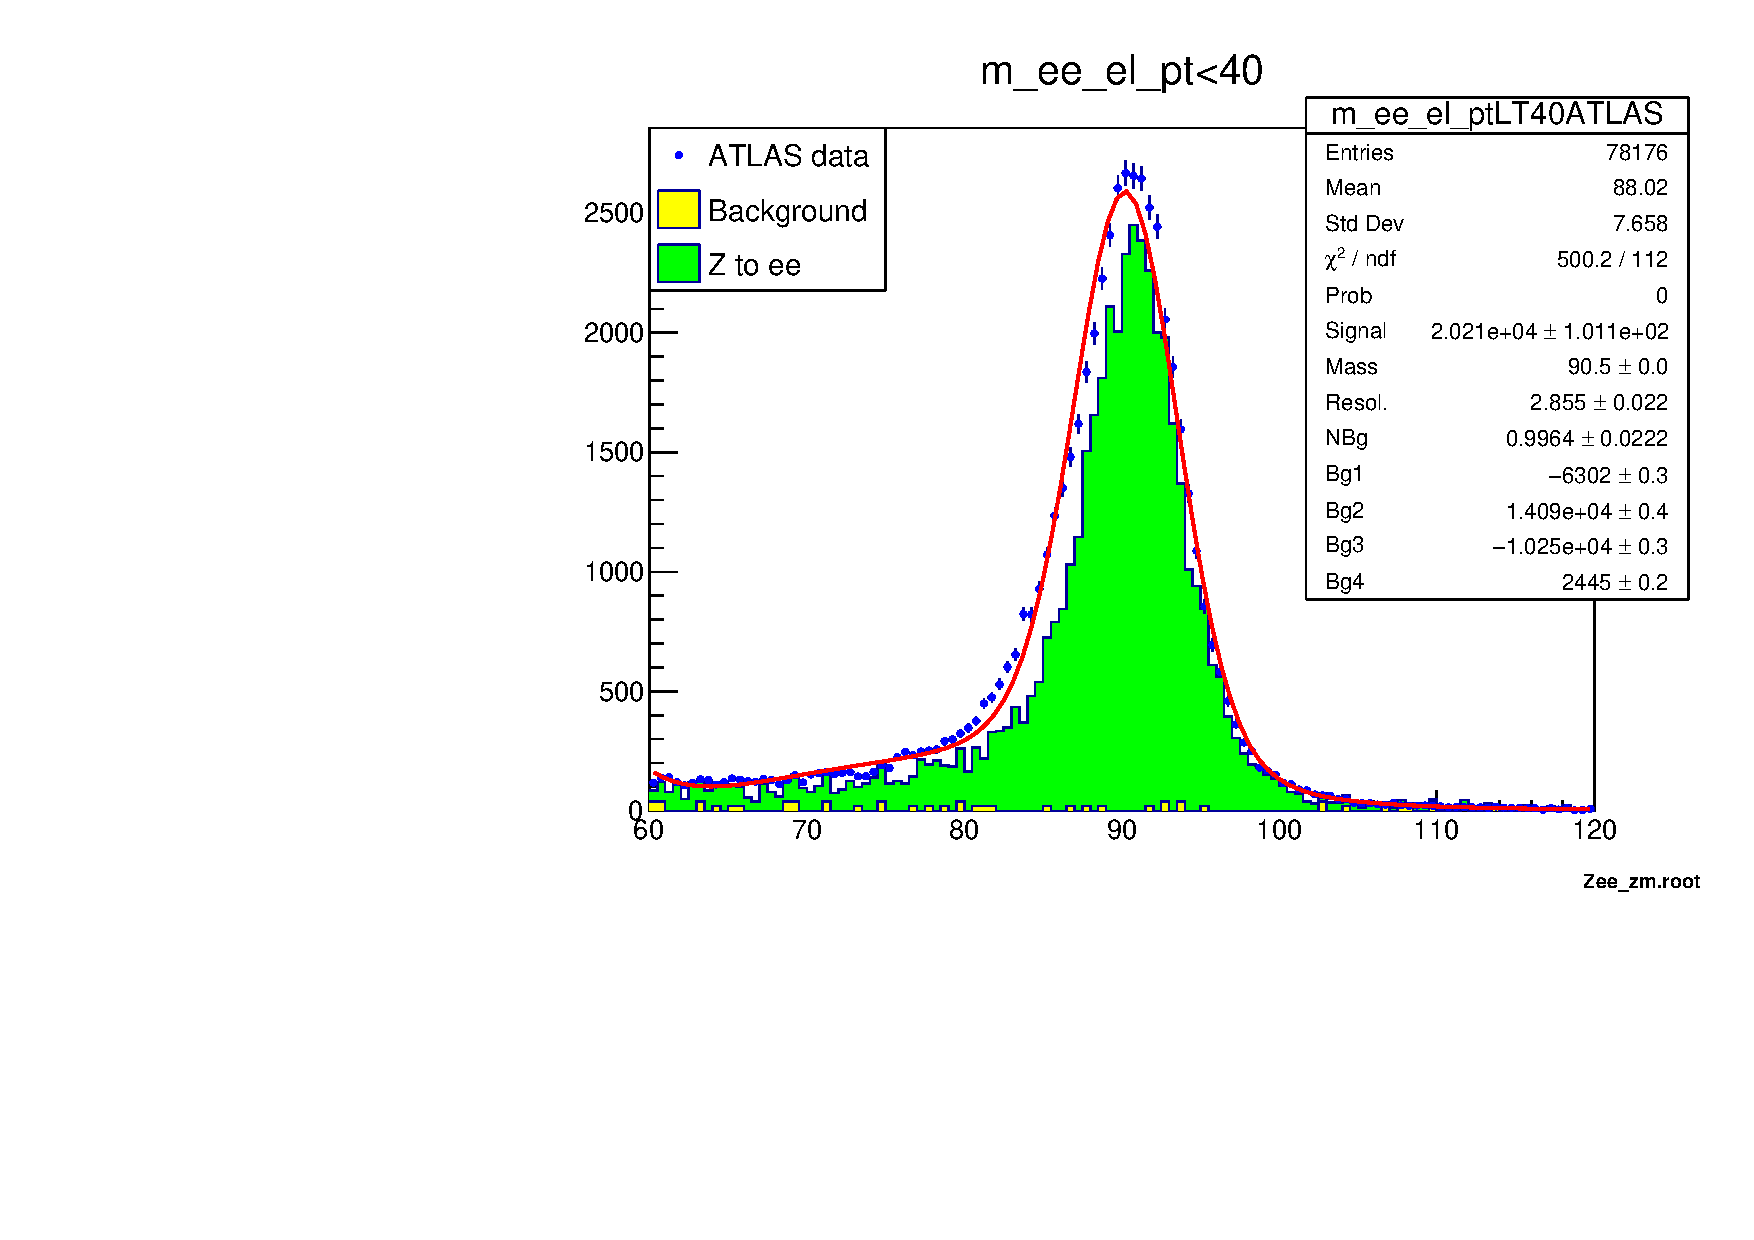
\includegraphics[width=\textwidth]{../W_mass/Z_mass_check_el_pt-cut-small.pdf}
            \subcaption{Fit to the $Z^0 \rightarrow e^+e^-$ canditates for $p_{T,e^{\pm}} < 40$\,GeV}
        \end{subfigure}
        \begin{subfigure}{0.5\textwidth}
            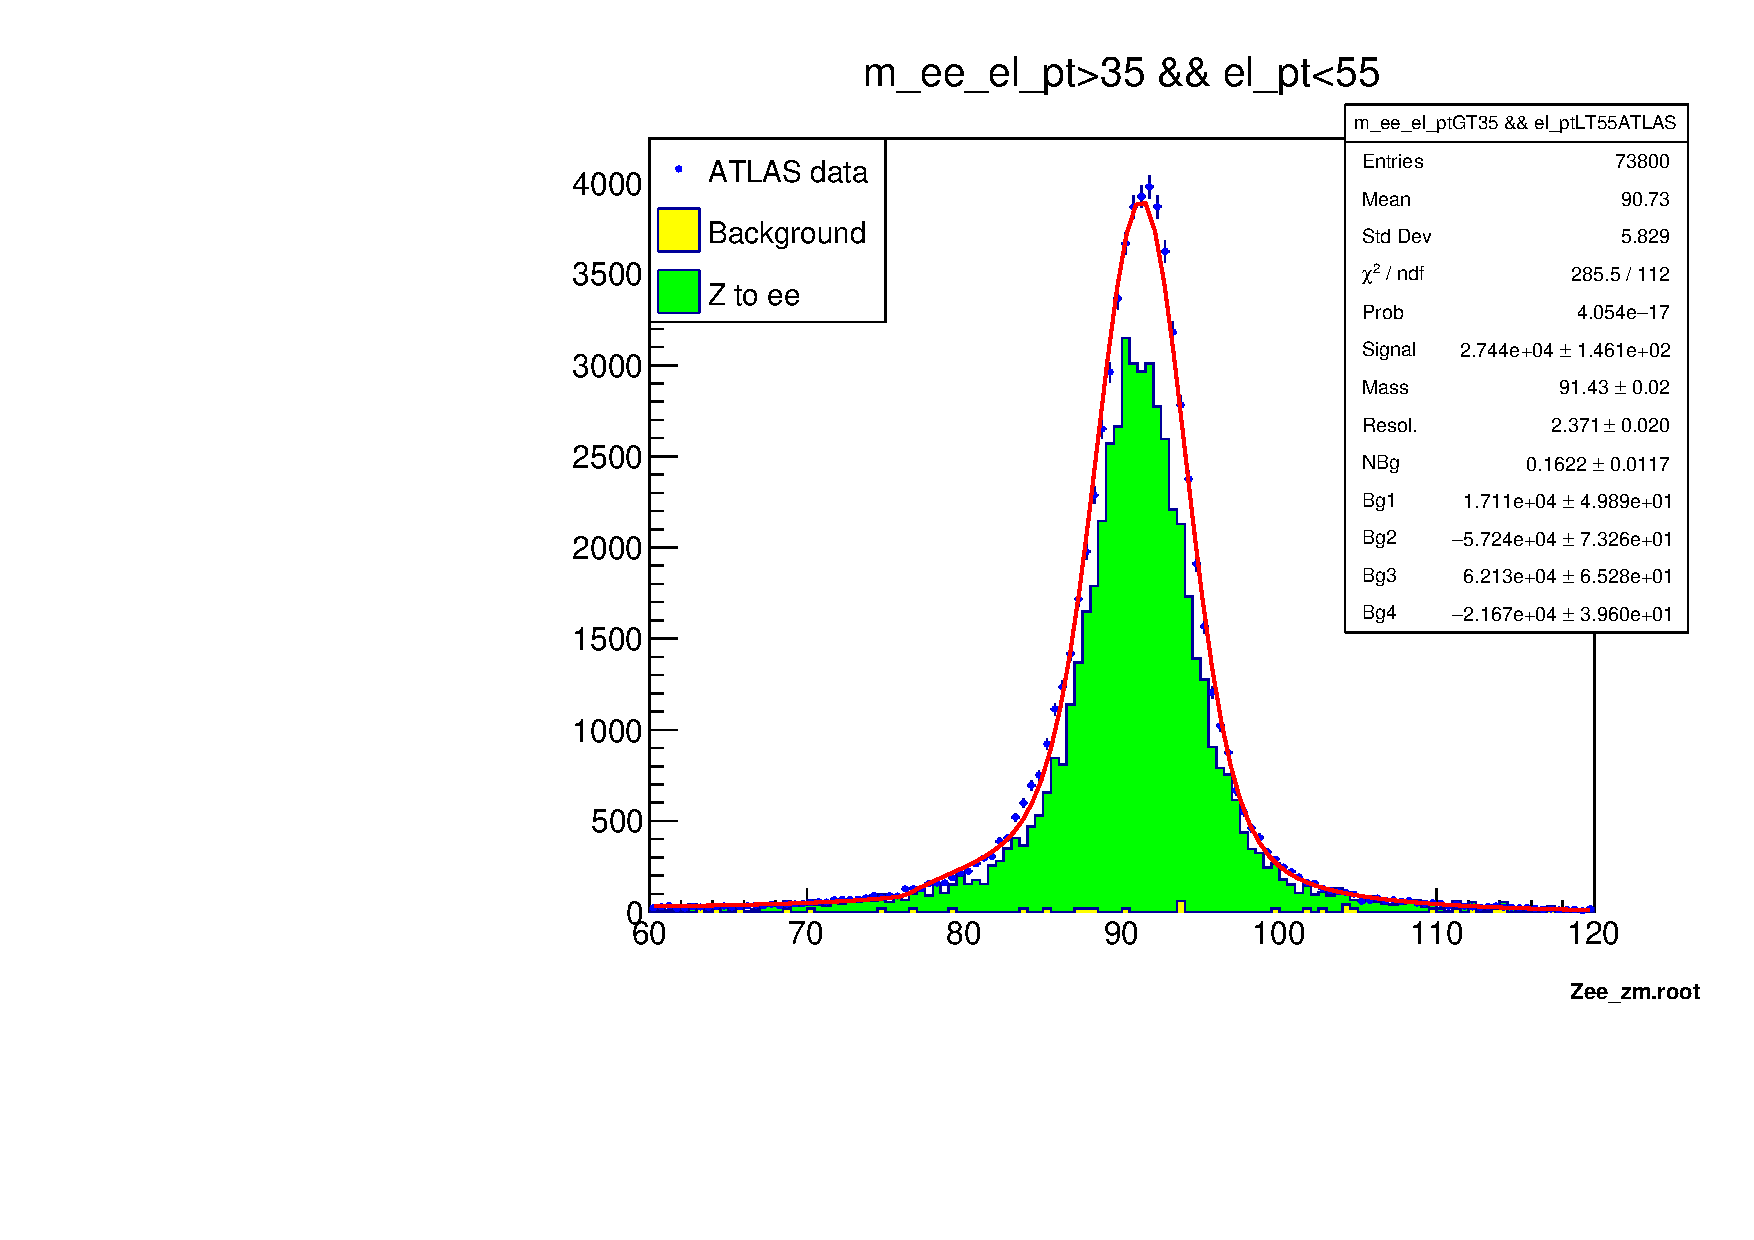
\includegraphics[width=\textwidth]{../W_mass/Z_mass_check_el_pt-cut-critical.pdf}
            \subcaption{Fit to the $Z^0 \rightarrow e^+e^-$ canditates for $35 < p_{T,e^{\pm}} < 55$\,GeV}
        \end{subfigure}
        \begin{subfigure}{0.5\textwidth}
            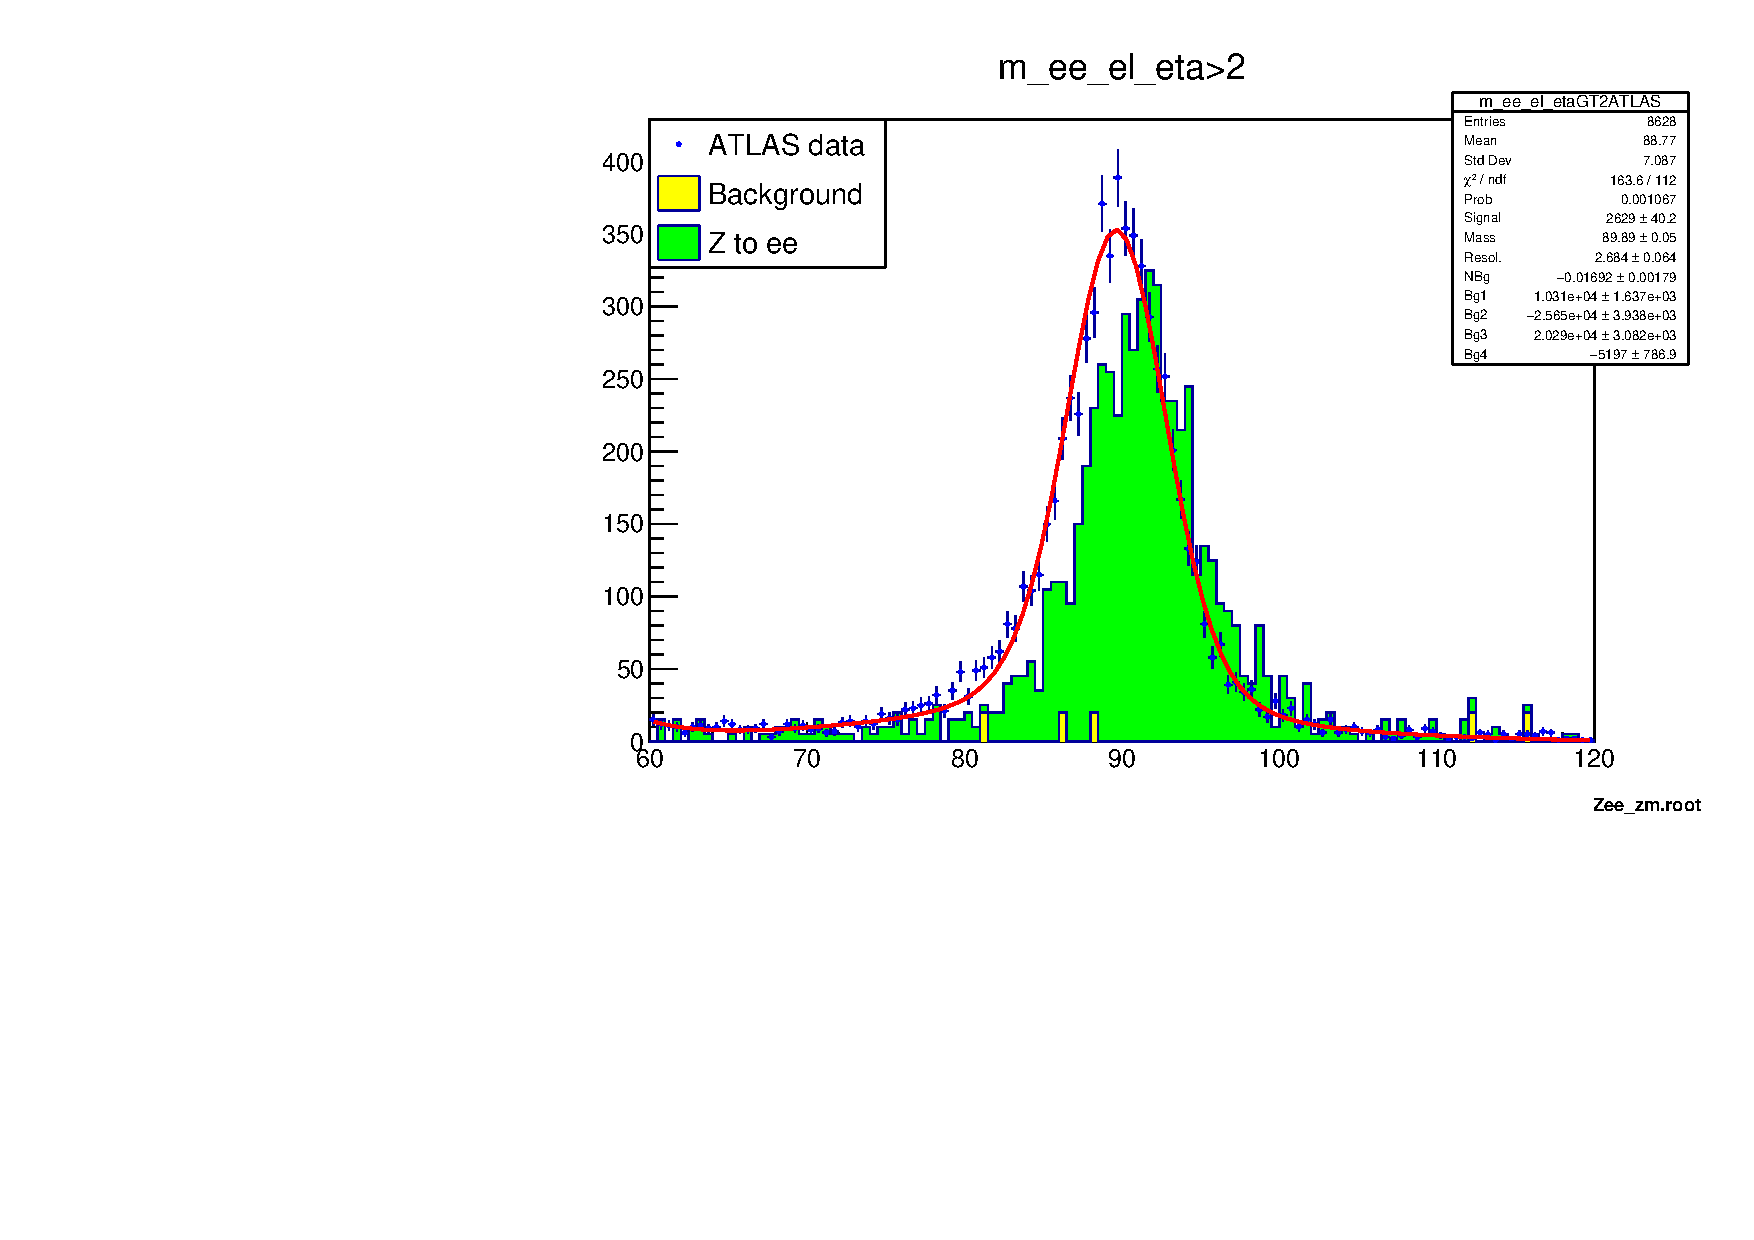
\includegraphics[width=\textwidth]{../W_mass/Z_mass_check_eta_large.pdf}
            \subcaption{Fit to the $Z^0 \rightarrow e^+e^-$ canditates for $\eta > 2$}
        \end{subfigure}
        \caption{Fitted $Z^0 \rightarrow e^+e^-$ data for different regions of the detector as well as different kinematic regions.}
        \label{fig:z-mass_check1}
    \end{figure}
    \begin{figure}
        \begin{subfigure}{0.5\textwidth}
            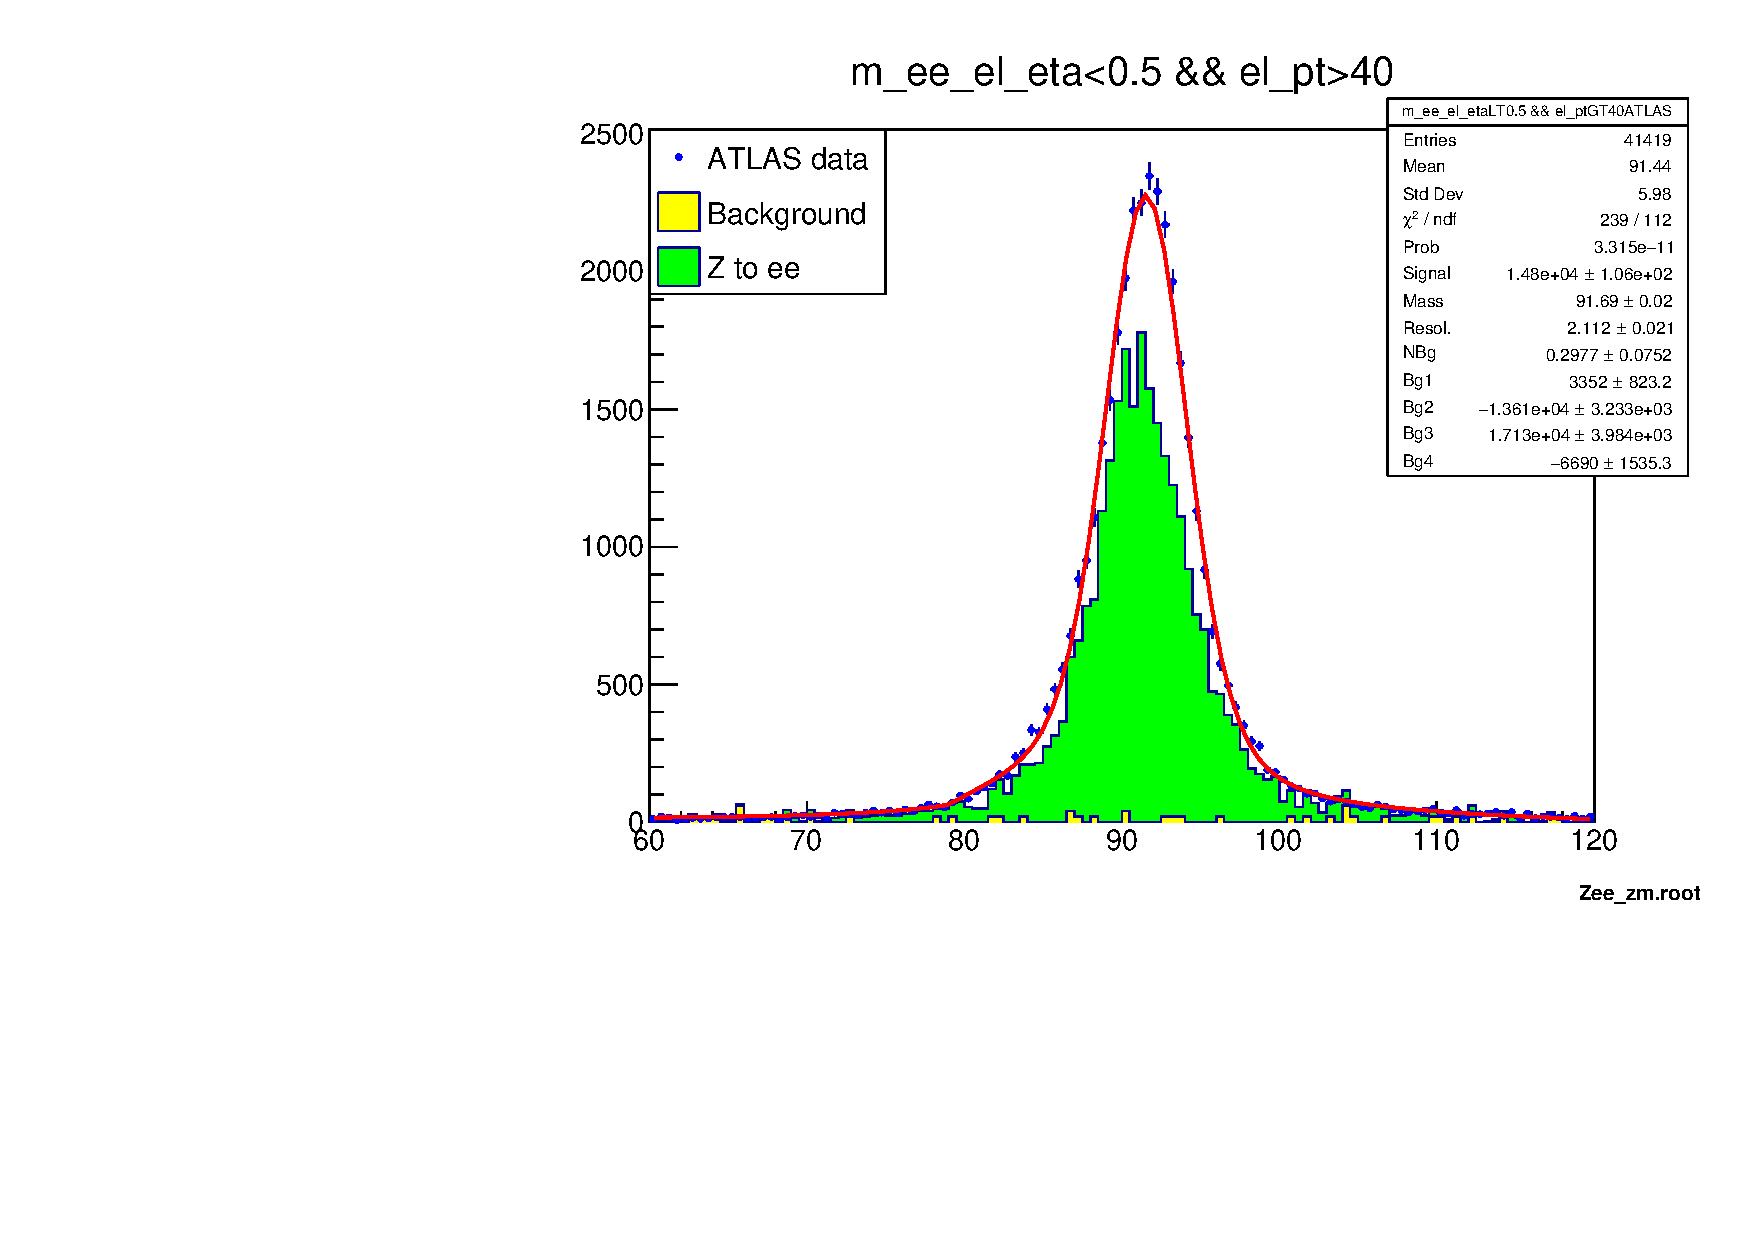
\includegraphics[width=\textwidth]{../W_mass/Z_mass_check_eta-small_pt-large.pdf}
            \subcaption{Fit to the $Z^0 \rightarrow e^+e^-$ canditates for $\eta < 0.5$ \& $p_{T,e^{\pm}} > 40$}
        \end{subfigure}
        \begin{subfigure}{0.5\textwidth}
            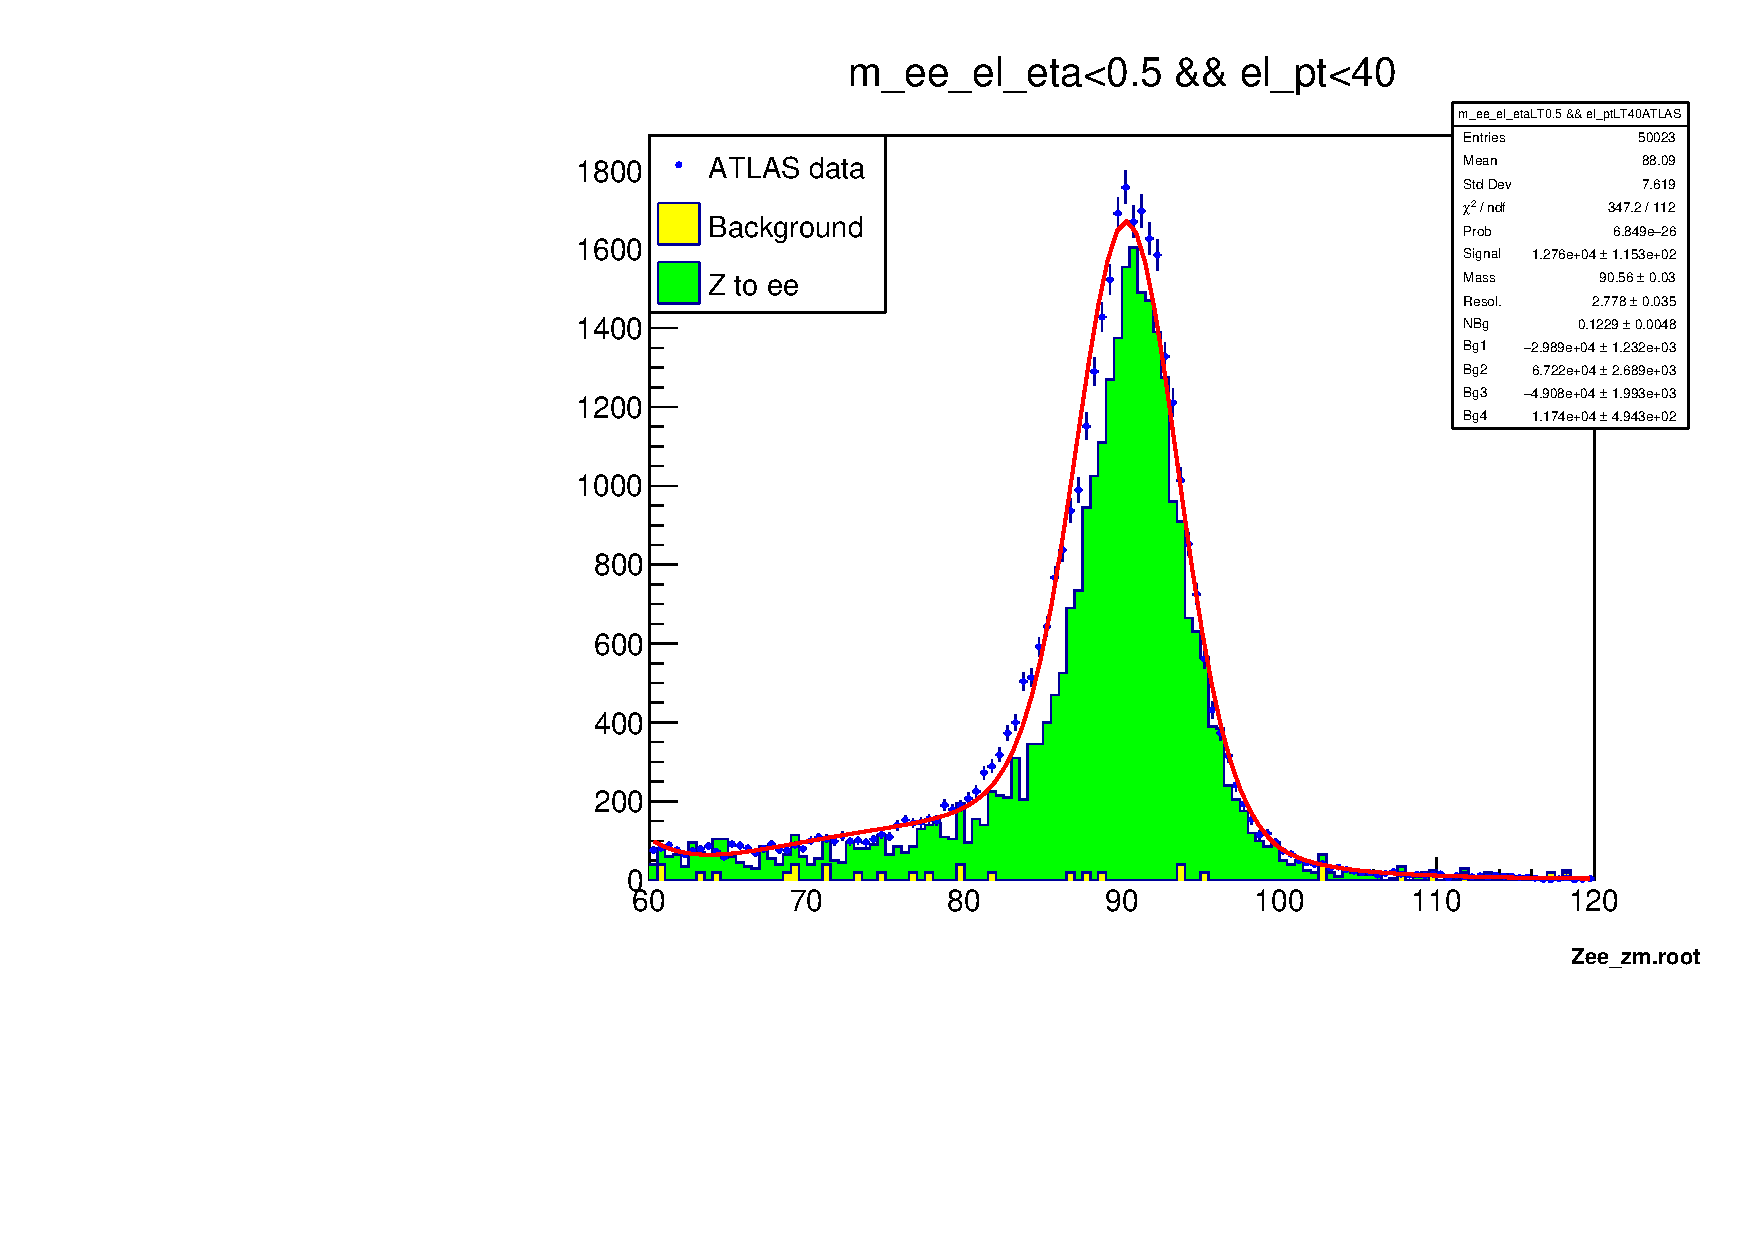
\includegraphics[width=\textwidth]{../W_mass/Z_mass_check_eta-small_pt-small.pdf}
            \subcaption{Fit to the $Z^0 \rightarrow e^+e^-$ canditates for $\eta < 0.5$ \& $p_{T,e^{\pm}} < 40$}
        \end{subfigure}
        \begin{subfigure}{0.5\textwidth}
            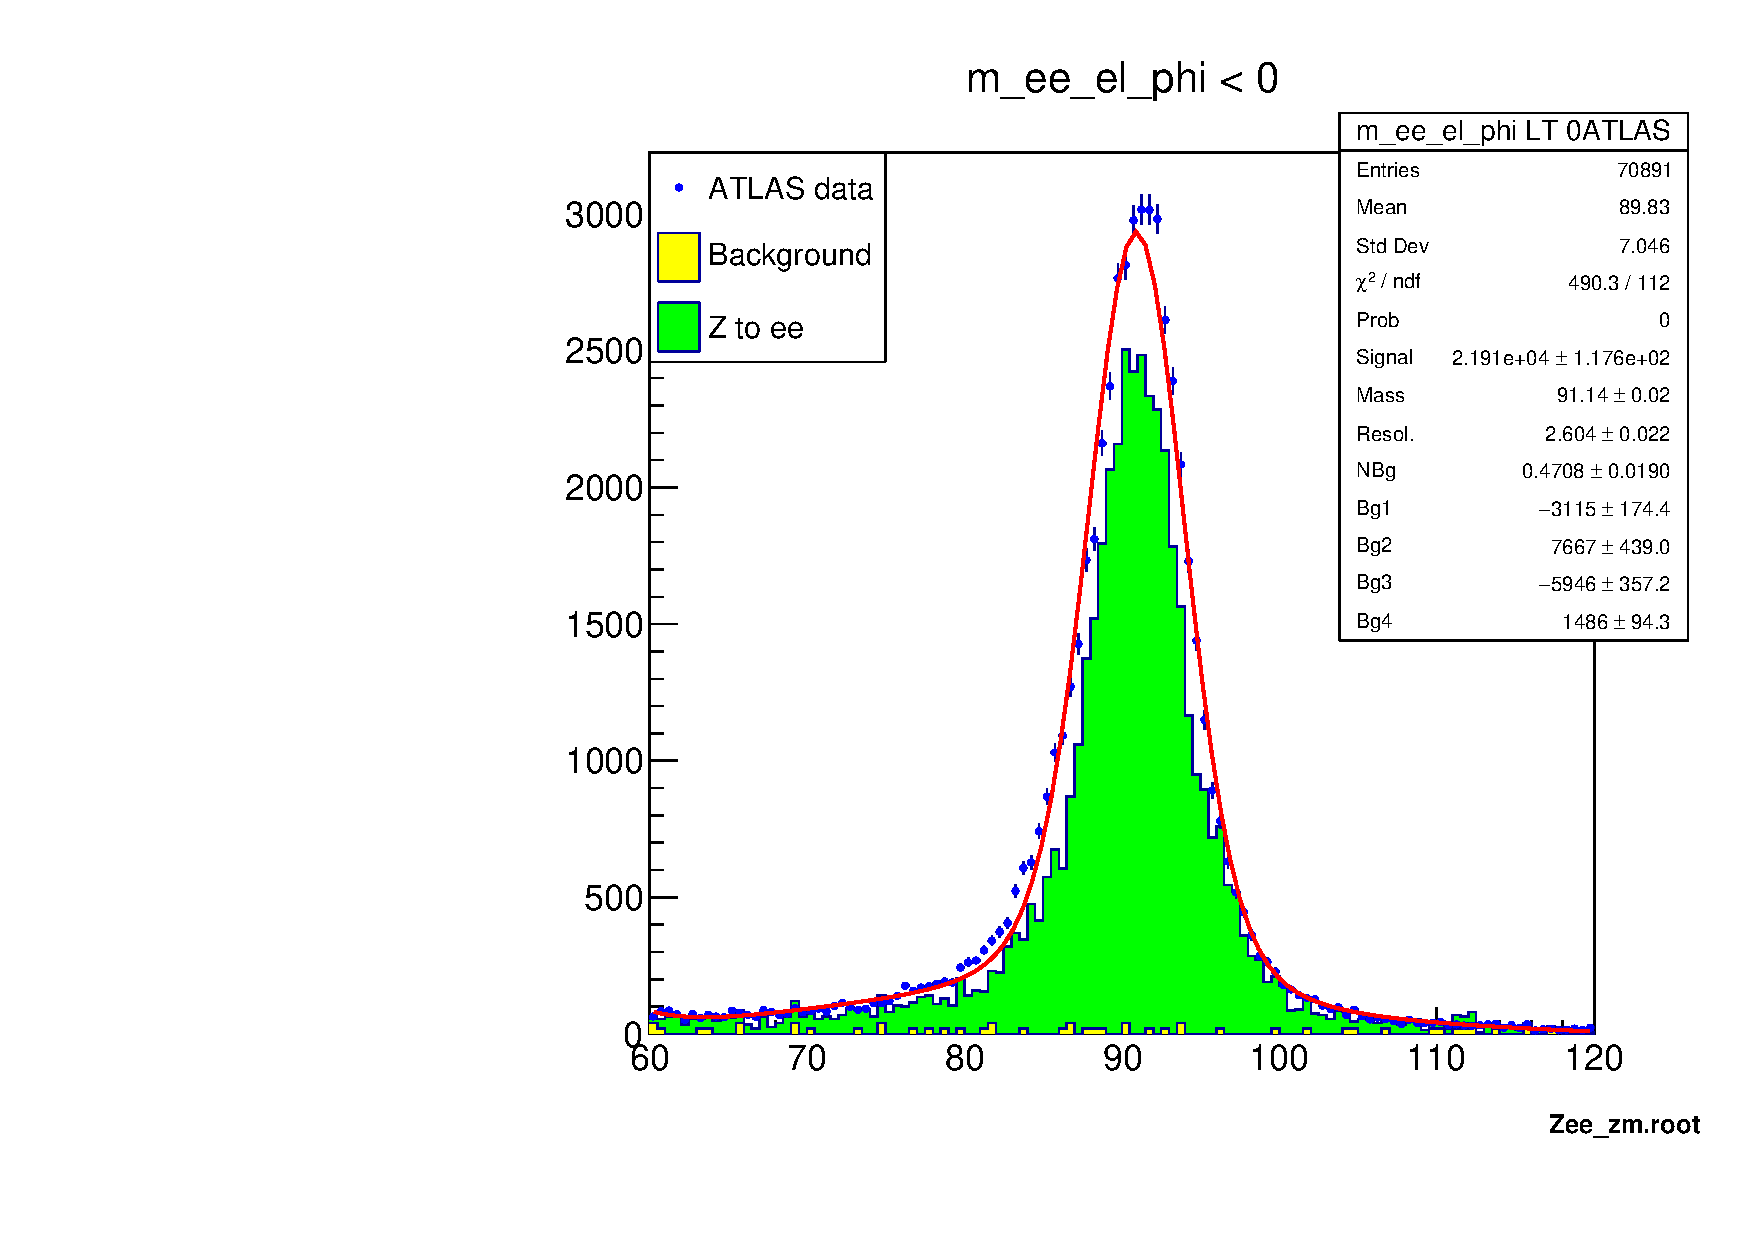
\includegraphics[width=\textwidth]{../W_mass/Z_mass_check_phi_negative.pdf}
            \subcaption{Fit to the $Z^0 \rightarrow e^+e^-$ canditates for $\phi < 0$}
        \end{subfigure}
        \begin{subfigure}{0.5\textwidth}
            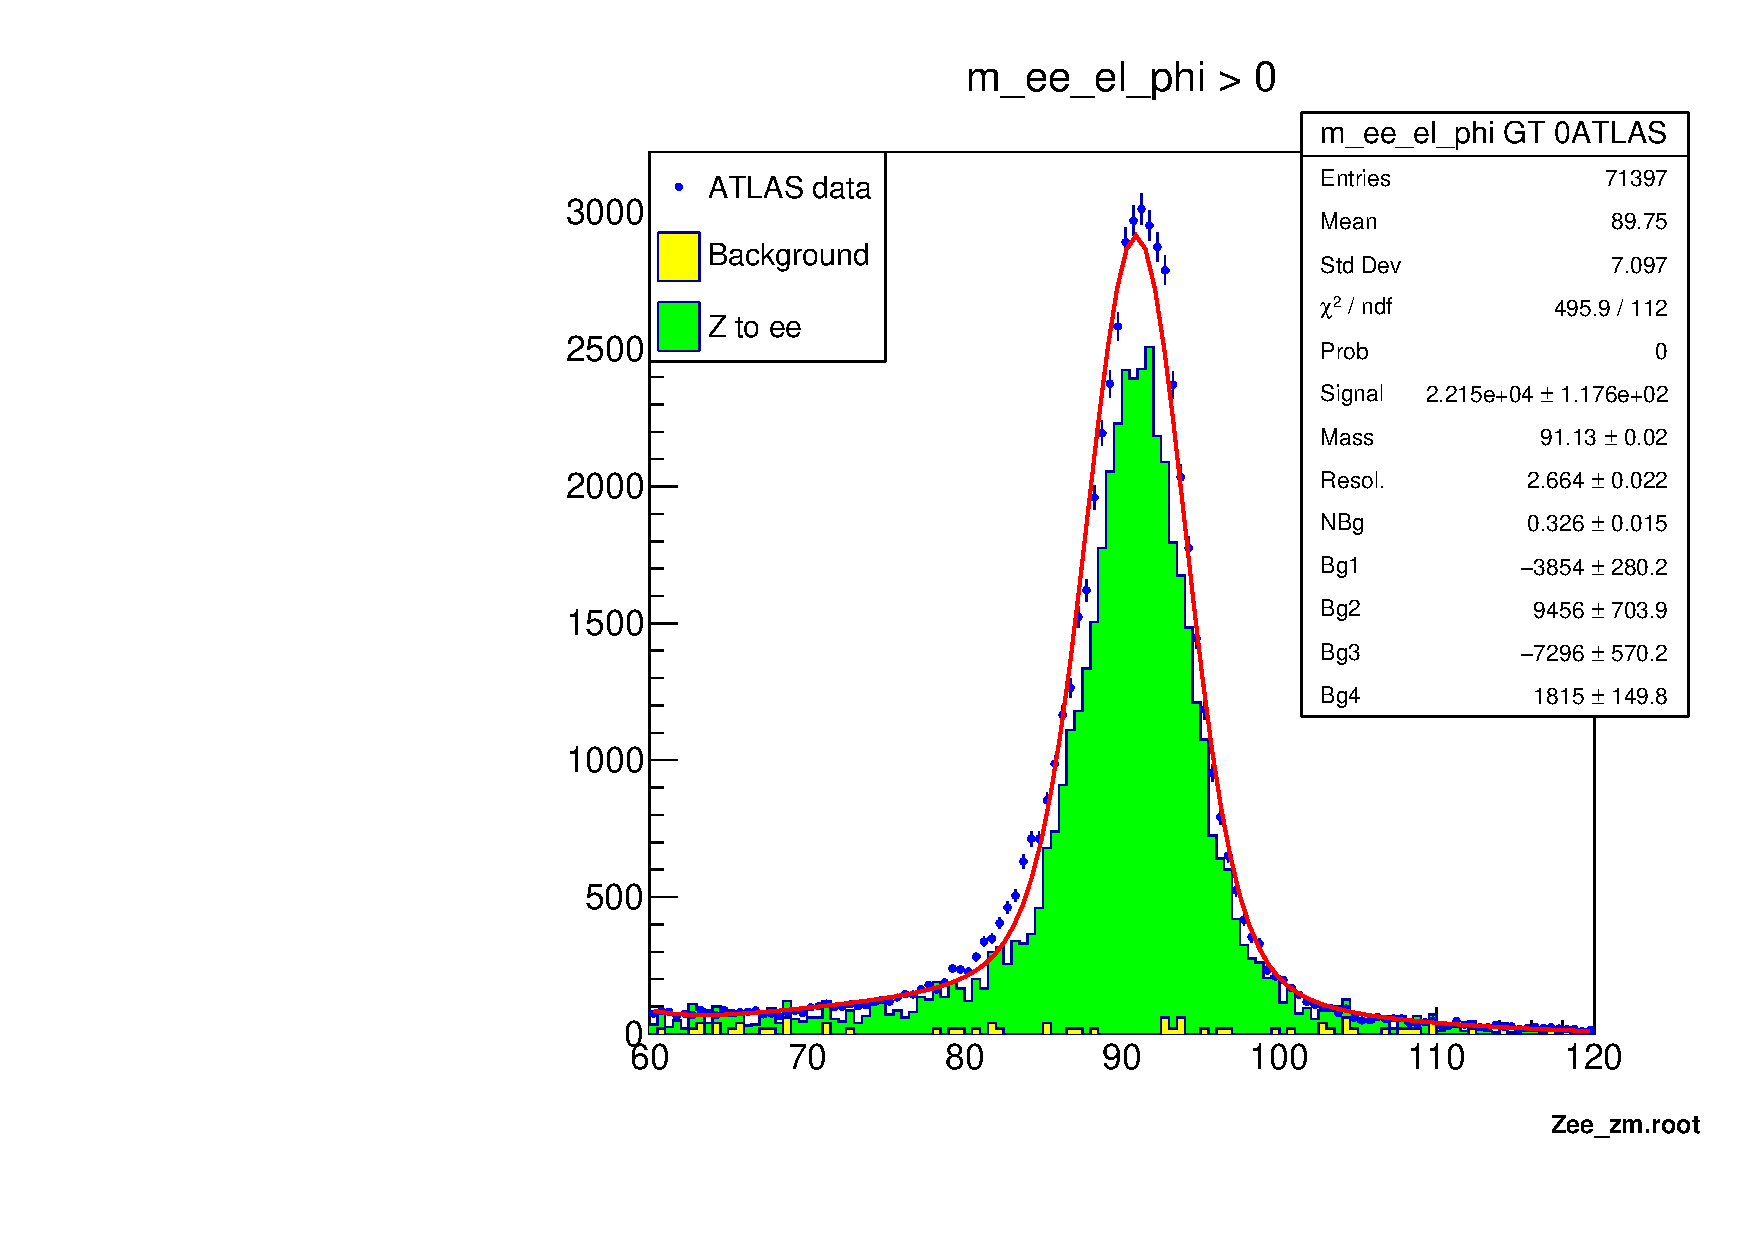
\includegraphics[width=\textwidth]{../W_mass/Z_mass_check_phi_positive.pdf}
            \subcaption{Fit to the $Z^0 \rightarrow e^+e^-$ canditates for $\phi > 0$}
        \end{subfigure}
        \caption{Fitted $Z^0 \rightarrow e^+e^-$ data for different regions of the detector as well as different kinematic regions.}
        \label{fig:z-mass_check2}
    \end{figure}


    \begin{table}
        \centering
        \begin{tabular}{cc}
            \toprule
            \toprule
            cut selection & $M_{Z^0,meas}$ / GeV \\
            \midrule
            $p_{T,e^{\pm}} > 40$ GeV & $91.71 \pm 0.02$  \\
            $p_{T,e^{\pm}} < 40$ GeV & $90.5 \pm 0.0$ \\
            $35 < p_{T,e^{\pm}} < 55$ GeV & $91.43 \pm 0.02$  \\
            $\eta > 2$ & $89.89 \pm 0.05$  \\
            $\eta < 0.5$ \& $p_{T,e^{\pm}} > 40$ & $91.69 \pm 0.02$  \\
            $\eta < 0.5$ \& $p_{T,e^{\pm}} < 40$ & $90.56 \pm 0.03$  \\
            $\phi < 0$ & $91.14 \pm 0.02$  \\
            $\phi > 0$ & $91.13 \pm 0.02$  \\
            \bottomrule
            \bottomrule
        \end{tabular}
        \caption{Measured $Z^0$ mass for different cut selections}
        \label{tab:z-masses}
    \end{table}
    Although there is some deviation from the literature value of the $Z^0$ mass, $m_{Z^0}^{lit} = (91.1880 \pm 0.0020)$\,GeV \cite{PDG2024}, overall the $Z^0$ masses are close
    to the literature value and deviate by less than 1\%. For large $\eta$ the deviation is a bit larger (1.), which is most likely due to the fact that the detector resolution is 
    best for particles which travel perpendicular to the beam line. The more forward the final particles are, the worse the detection efficiency resolution get. 

\subsection{QCD scale factor and Kinematic Variables}
    \label{sec:qcd_factor/variables}
    In order to achieve an accurate measurement of the W-mass, the background processes at ATLAS have to be taken into consideration.
    At LHC, proton proton collisions cause the measured events, therefore the background coming from QCD processes is large. This causes a problem,
    since the final products of the $W \rightarrow e\nu$ events we use to measure the W-mass are leptons which do not interact with the strong interaction.
    This makes the simulation of a QCD background for the $W \rightarrow e\nu$ events difficult. In order to solve this problem, the QCD background is extracted
    from the data. In order to scale the data correctly, a QCD scale factor is used, since the integrated luminosity of the background is not measured and therefore
    unknown. In order to get an understanding of the QCD scale factor and its effect on the data, different kinematic values are be plotted for different 
    QCD scale factors.

\subsubsection{Kinematic Variables}
    \label{sec:variables}
    In order to get a feeling for the QCD scale factor and estimate its optimal value, different kinematic Variables are analyzed.
    The chosen kinematic variables are \texttt{el\_pt} (the transverse momentum of the electron), \texttt{etmis} (missing transverse energy/momentum),
    \texttt{njet} (number of jets in the event) and \texttt{ptw} (transverse momentum of the W boson). The distributions of these different variables
    for a scale factor of 1 (meaning no scaling) can be seen in figure \ref{fig:qcd1}. From figure \ref{fig:qcd1} it is obvious that the ATLAS data does not agree very well with 
    the simulations. In order to solve this, the QCD scale factor was set to different values whilst looking at the distributions until the agreement between real and simulated data
    was optimal by eye. Compromises were necessary, since the alignment between real data and simulated data was unequal for different regions. 
    After some trial and error, the optimal QCD scale factors the four mentioned kinematic variables were chosen as:
    \begin{table}[H]
        \centering
        \begin{tabular}{cc}
            \toprule
            Variable & QCD scale factor \\
            \midrule
            \texttt{etmis}   &  $0.30 \pm 0.05$ \\ 
            \texttt{el\_pt}  &  $0.35 \pm 0.07$ \\
            \texttt{nejt}    &  $0.46 \pm 0.08$ \\
            \texttt{ptw}     &  $0.42 \pm 0.06$ \\
            \bottomrule
        \end{tabular}
        \caption{Optimal QCD scale factors for each of the examined kinematic variables.}
        \label{tab:scale_factors}
    \end{table}
    The errors were chosen to account for the previously mentioned problem, that the data aligned unequally well with the simulated data in different regions of the distributions.
    Therefore the errors were chosen, such that at the end of the error interval, the alignment was best in one region whilst the disalignment in the rest of the distribution was
    still decent. 
    Overall the kinematic variables display the expected behavior. The transverse momentum of the W-boson \texttt{ptw} is mostly small, meaning less than ca. 30\,GeV.
    When looking at the electron transverse momentum \texttt{el\_pt}, the $W \rightarrow e\nu$ events display a peak between 40 and 50\,GeV which is expected since this 
    is around half the mass of the W-boson, which is coming from the Jacobi peak \cite{atlaslabmanual}. The increase towards lower $p_T$ is mostly due to QCD background.
    When looking at the missing transverse momentum \texttt{etmis} the distribution behaves similarly to the electron transverse momentum \texttt{el\_pt}, which is expected.
    Since the transverse momentum of the W-bosons is mostly small, compared to that of the from the decay resulting electron and neutrino, due to momentum conservation, the 
    electron and the neutrino get approximately half the W-boson mass as energy. It is therefore expected that both these distributions, when disregarding the background, 
    feature a peak located around the W-boson mass. The distribution 
    \begin{figure}
        \begin{subfigure}{0.5\textwidth}
            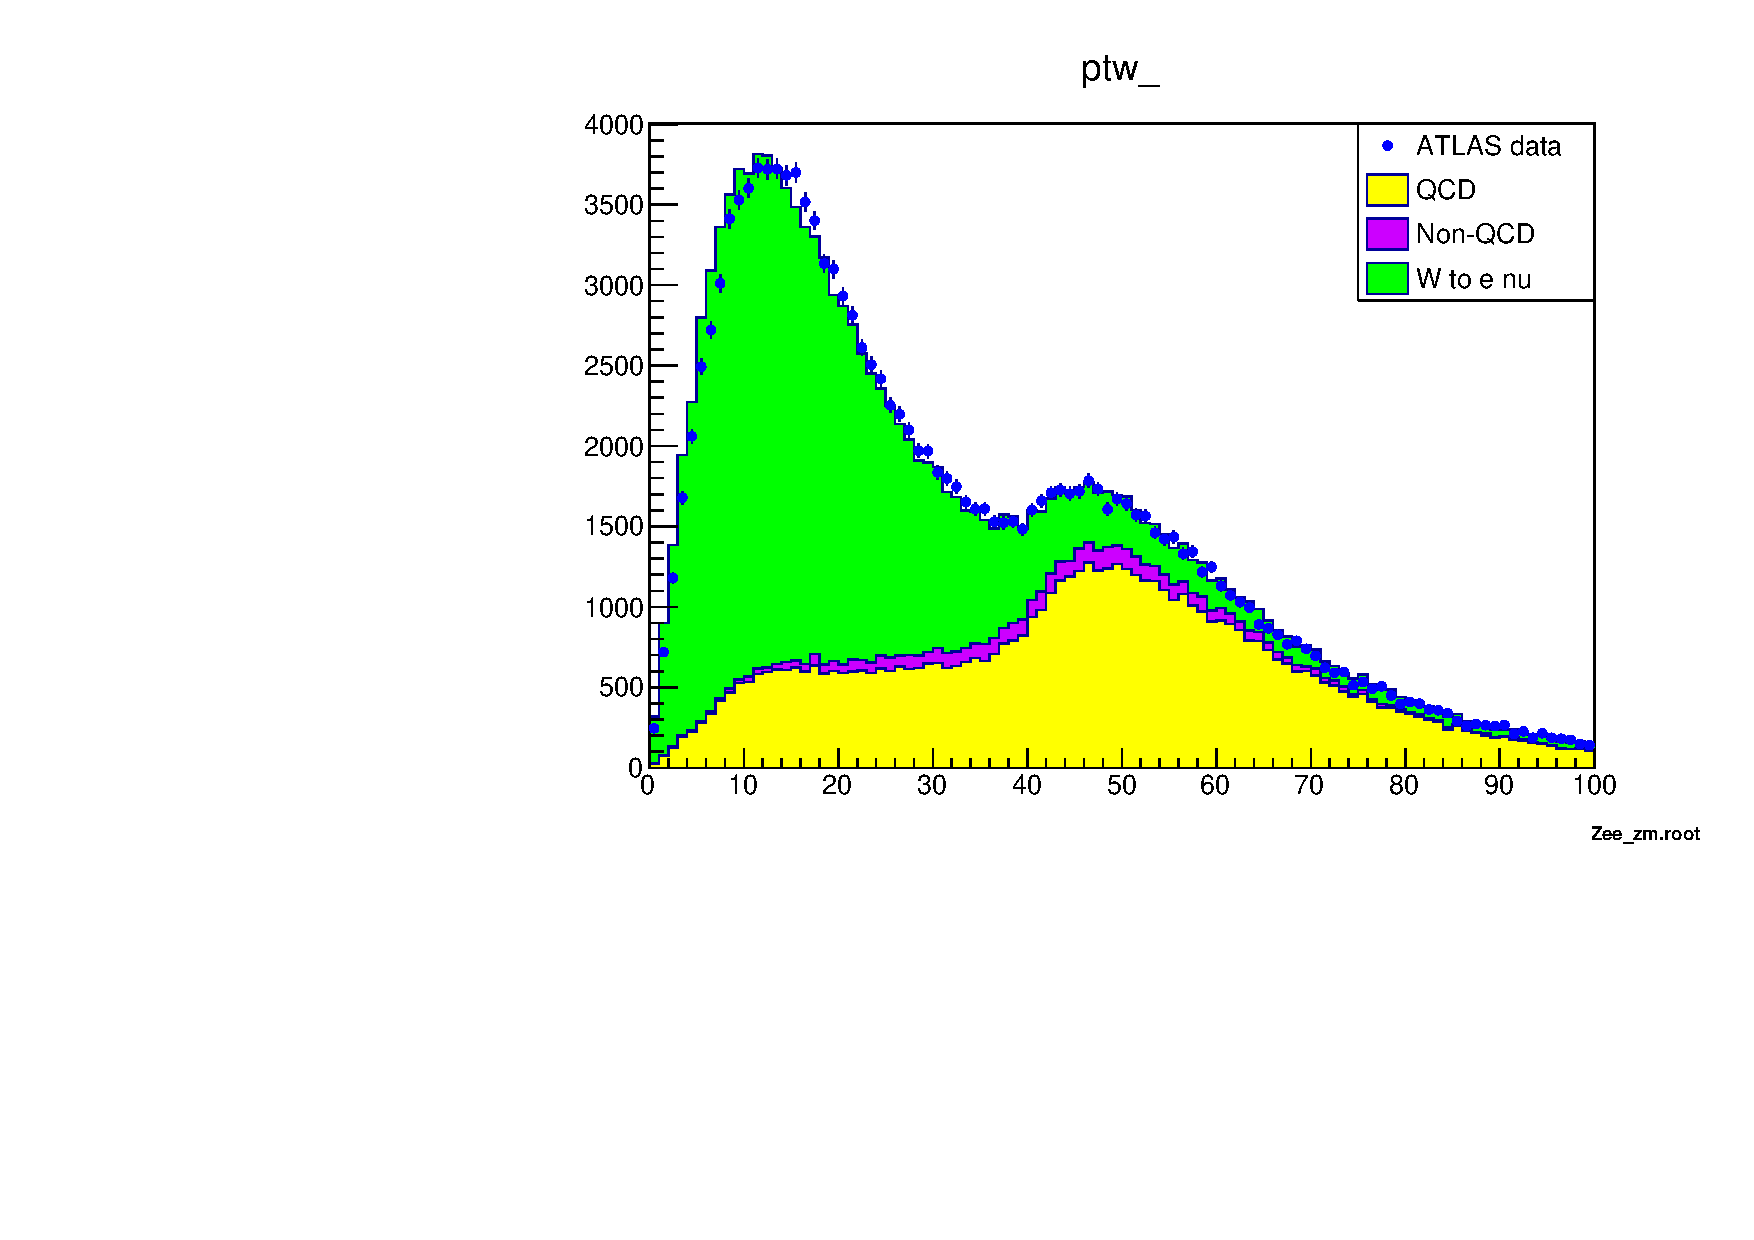
\includegraphics[width=\textwidth]{../W_mass/ptw_100_0_100_qcd0-42.pdf}
        \end{subfigure}
        \begin{subfigure}{0.5\textwidth}
            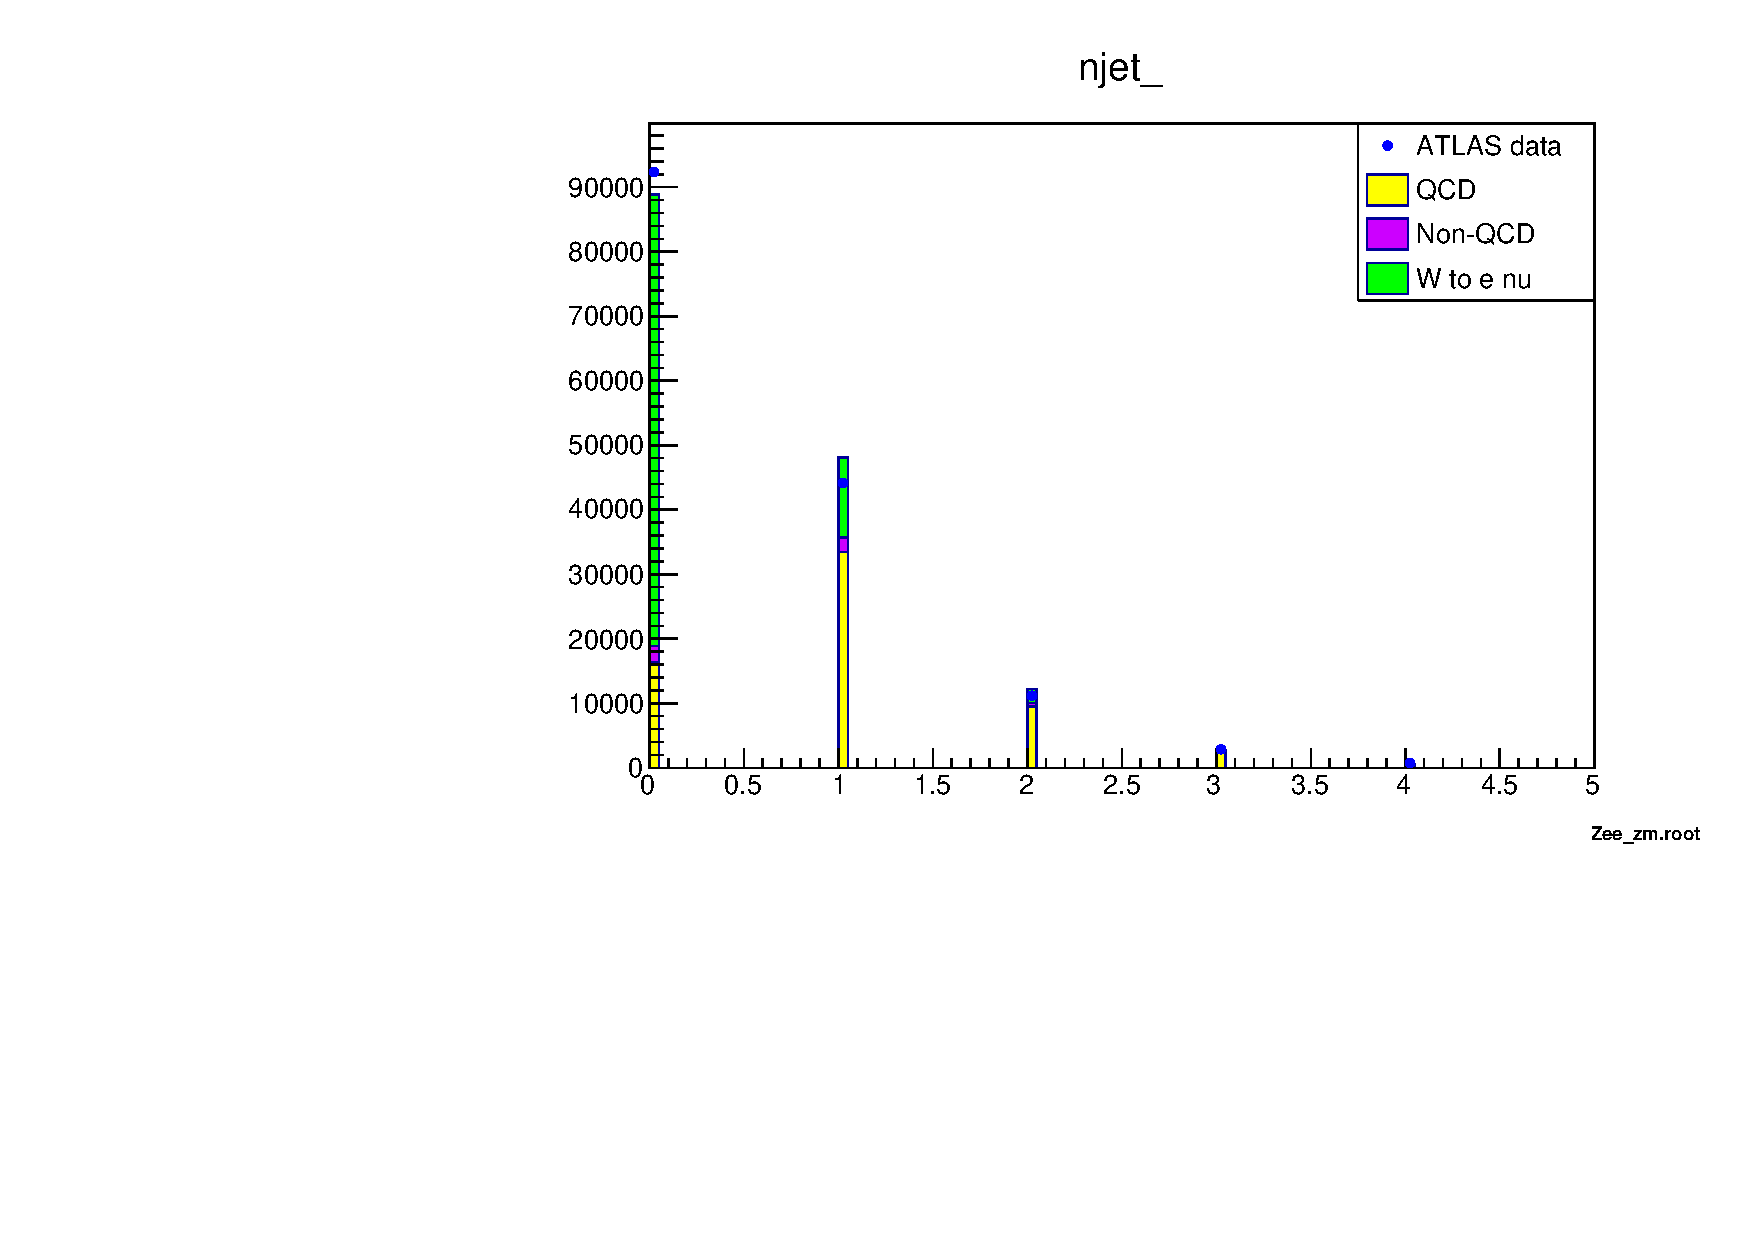
\includegraphics[width=\textwidth]{../W_mass/njet_100_0_5_qcd0-42.pdf}
        \end{subfigure}
        \begin{subfigure}{0.5\textwidth}
            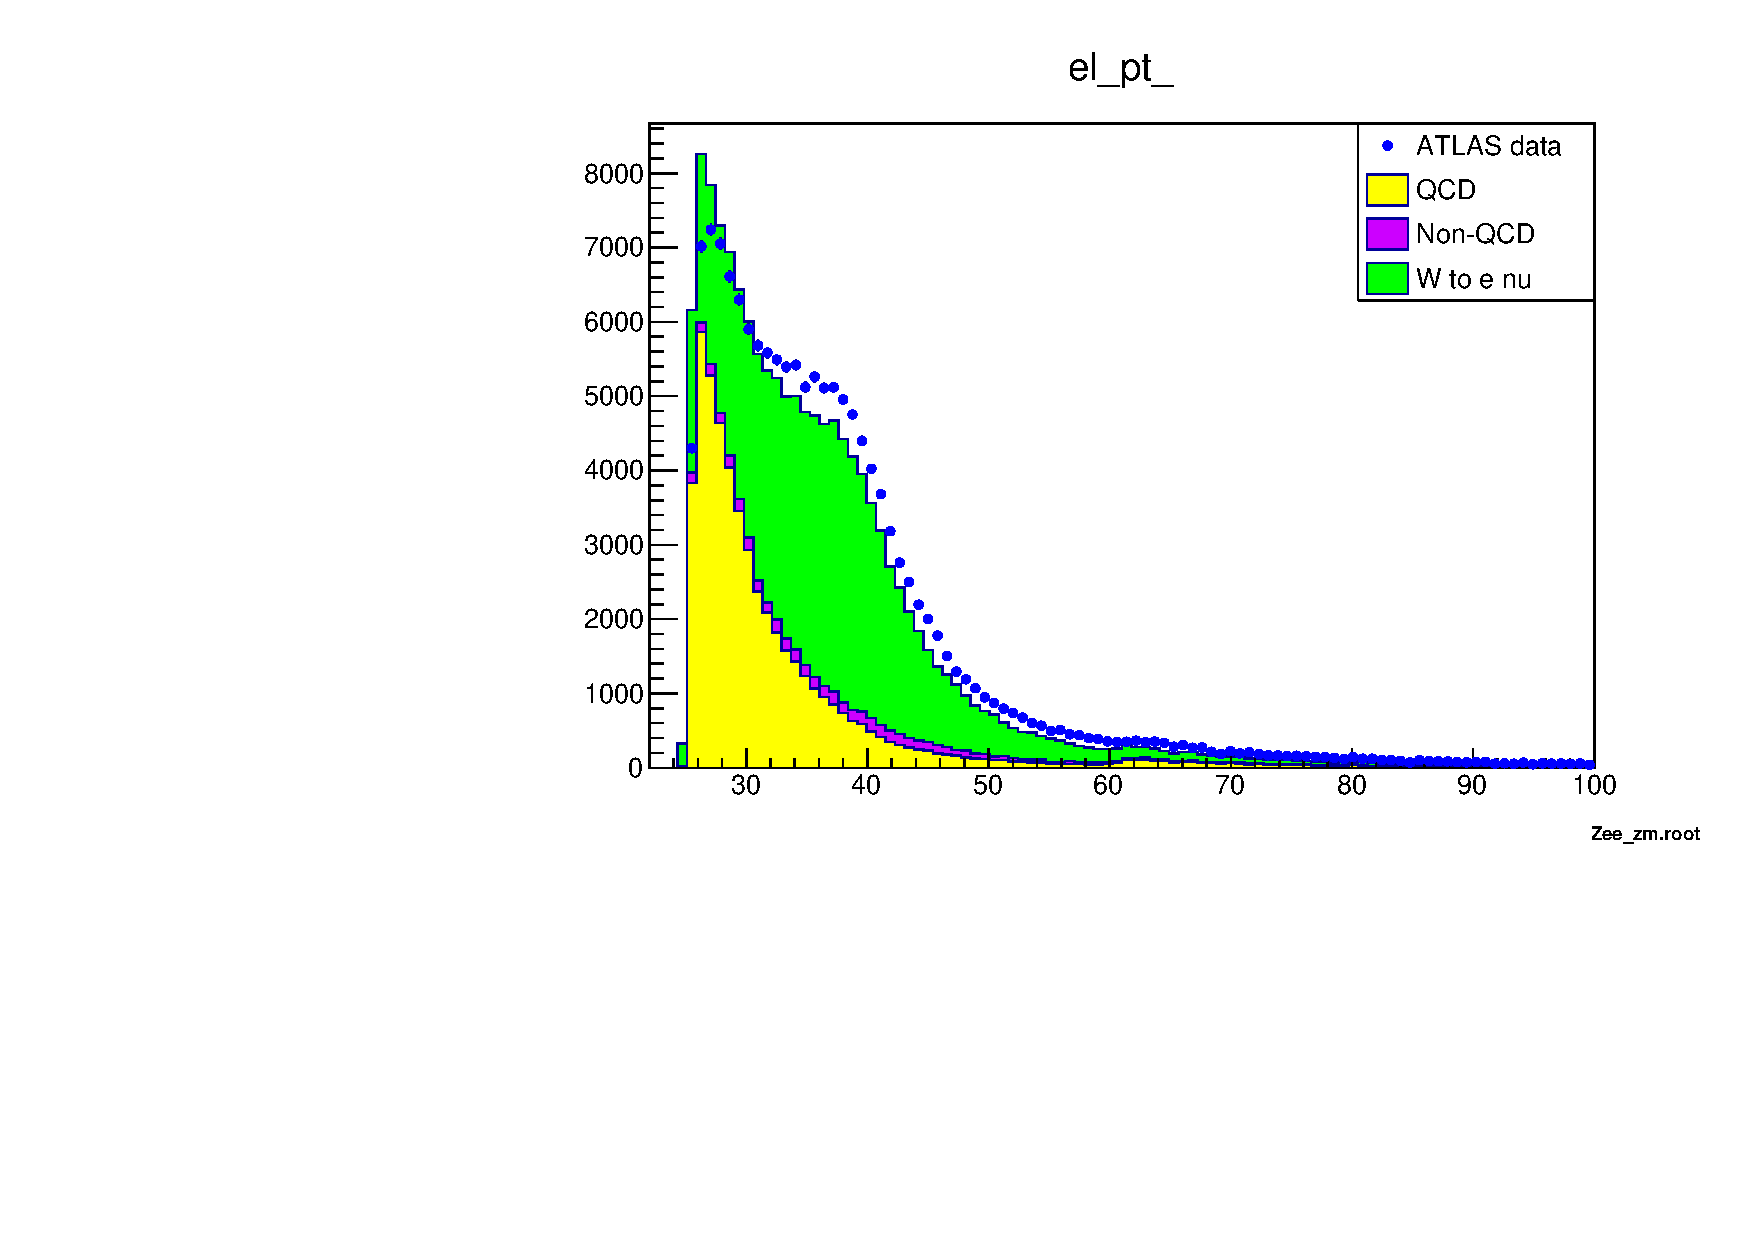
\includegraphics[width=\textwidth]{../W_mass/elpt_100_25_100_qcd0-35.pdf}
        \end{subfigure}
        \begin{subfigure}{0.5\textwidth}
            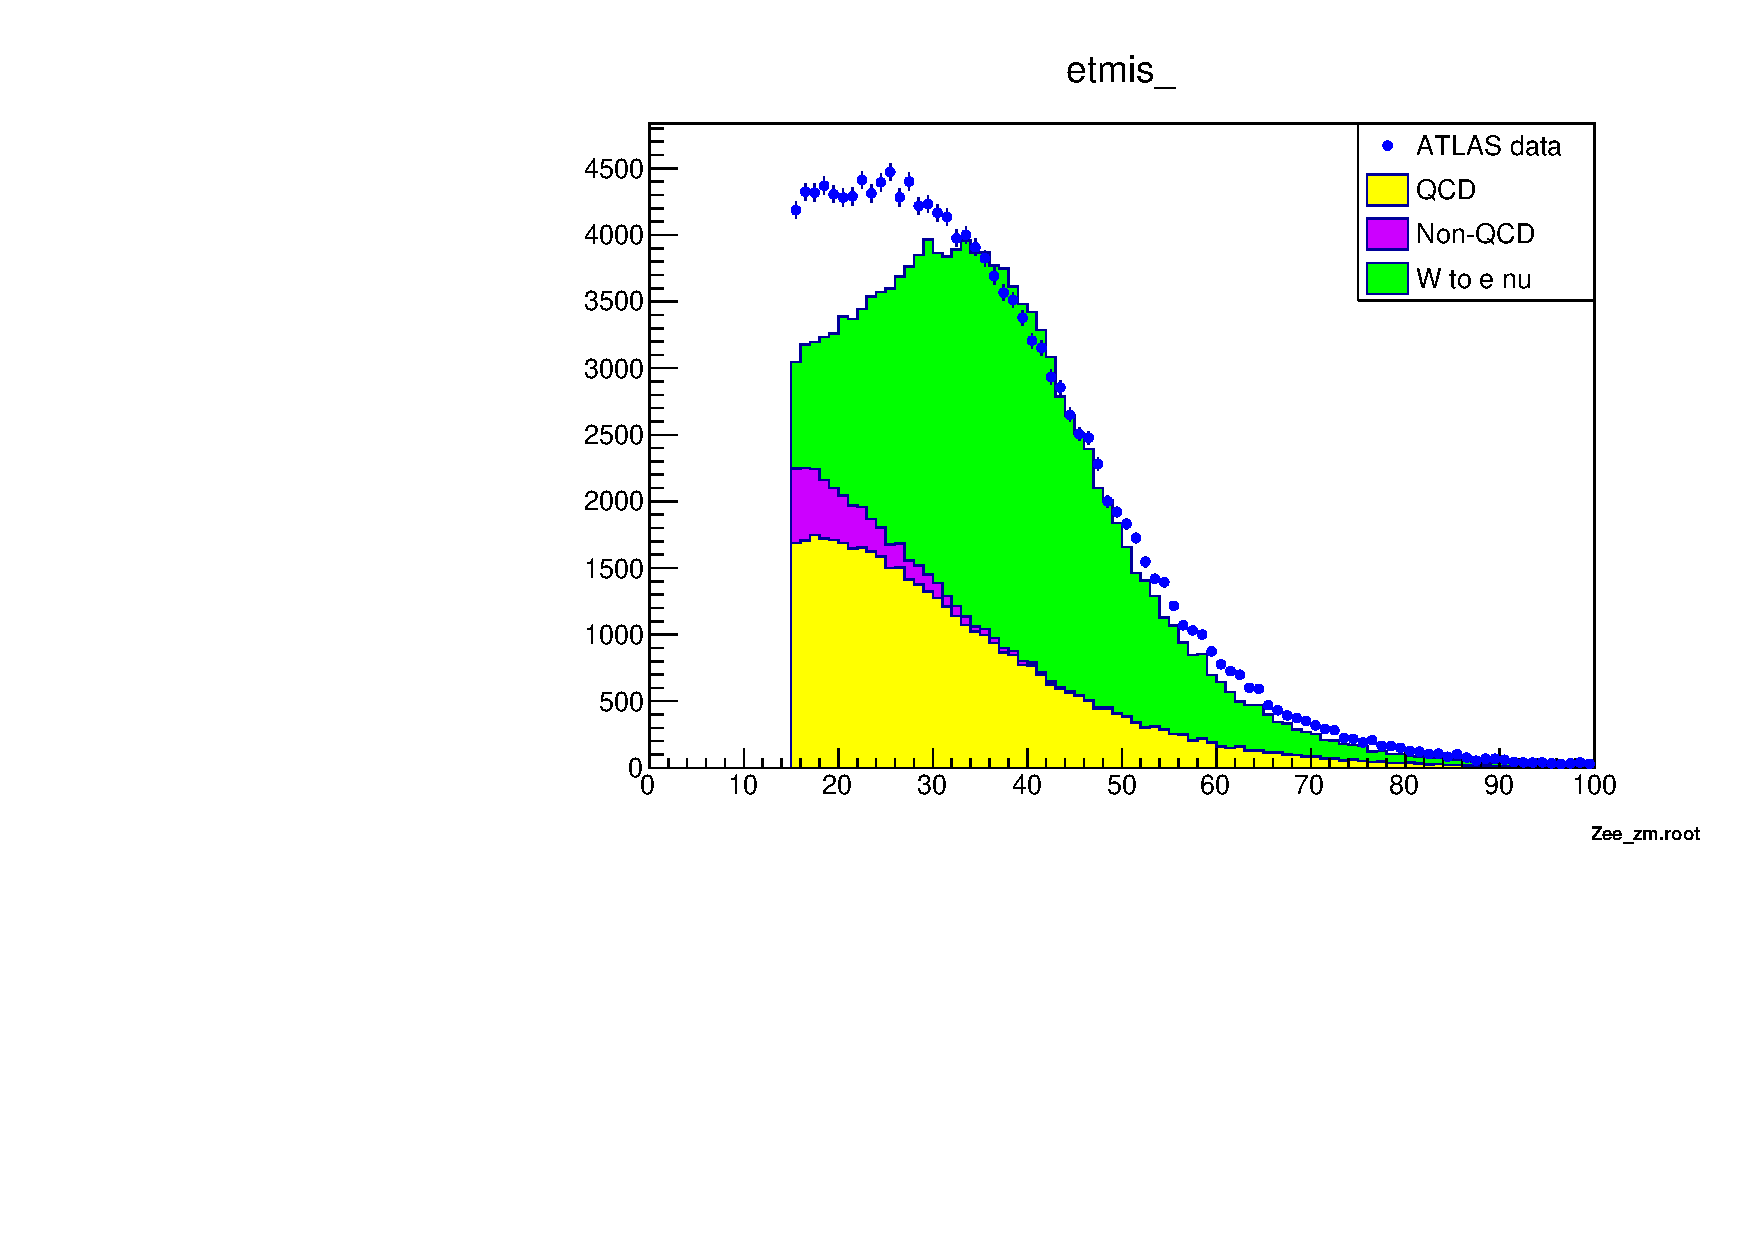
\includegraphics[width=\textwidth]{../W_mass/etmis_100_0_100_qcd0-3.pdf}
        \end{subfigure}
        \caption{Distributions of the kinematic variables \texttt{ptw}, \texttt{njet}, \texttt{el\_pt} and \texttt{etmis} for the QCD factors mentioned in table \ref{tab:scale_factors}}
        \label{fig:qcd-final}
    \end{figure}
    In the next step, the distribution of $p_T^W$ is analyzed for events with different jet multiplicities. The corresponding histograms are displayed in figure \ref{fig:ptw_jets}.
    A clear trend is observed: the signal-to-background ratio decreases as the number of jets increases.
    This behavior aligns with the jet multiplicity distribution shown previously in figure \ref{fig:qcd-final}.

    For events with zero jets, the signal is dominant at low $p_T^W$, peaking around 10-15\,GeV. This is expected, as there are no jets present to impart recoil to the W boson.
    However, when considering events with one jet, the signal drops significantly, and the previously observed peak at low $p_T^W$ disappears.
    Instead, the signal appears relatively flat in the low to mid-$p_T^W$ range and then declines at higher values.
    This can be explained by the presence of one jet in these signal events, which imparts recoil to the W boson.
    Although the jet direction is unknown, assuming an isotropic distribution, this results in a roughly uniform $p_T^W$ distribution.
    Lower $p_T^W$ values correspond to a forward jet recoil, while mid to high $p_T^W$ suggests more transverse recoil.

    The background shows a noticeable increase around 50\,GeVGeV. This could be related to the W boson mass, as the peak occurs slightly above half its mass,
    although other factors may also contribute.

    As the number of jets increases further, the signal continues to diminish while the background becomes more dominant.
    The background still peaks around 50\,GeV, but the overall number of events decreases.
    This trend is consistent with expectations: the original process does not favor the presence of jets,
    and the likelihood of additional (radiated) jets decreases with increasing event complexity, due to a reduction in available vertices.
    \begin{figure}
        \begin{subfigure}{0.5\textwidth}
            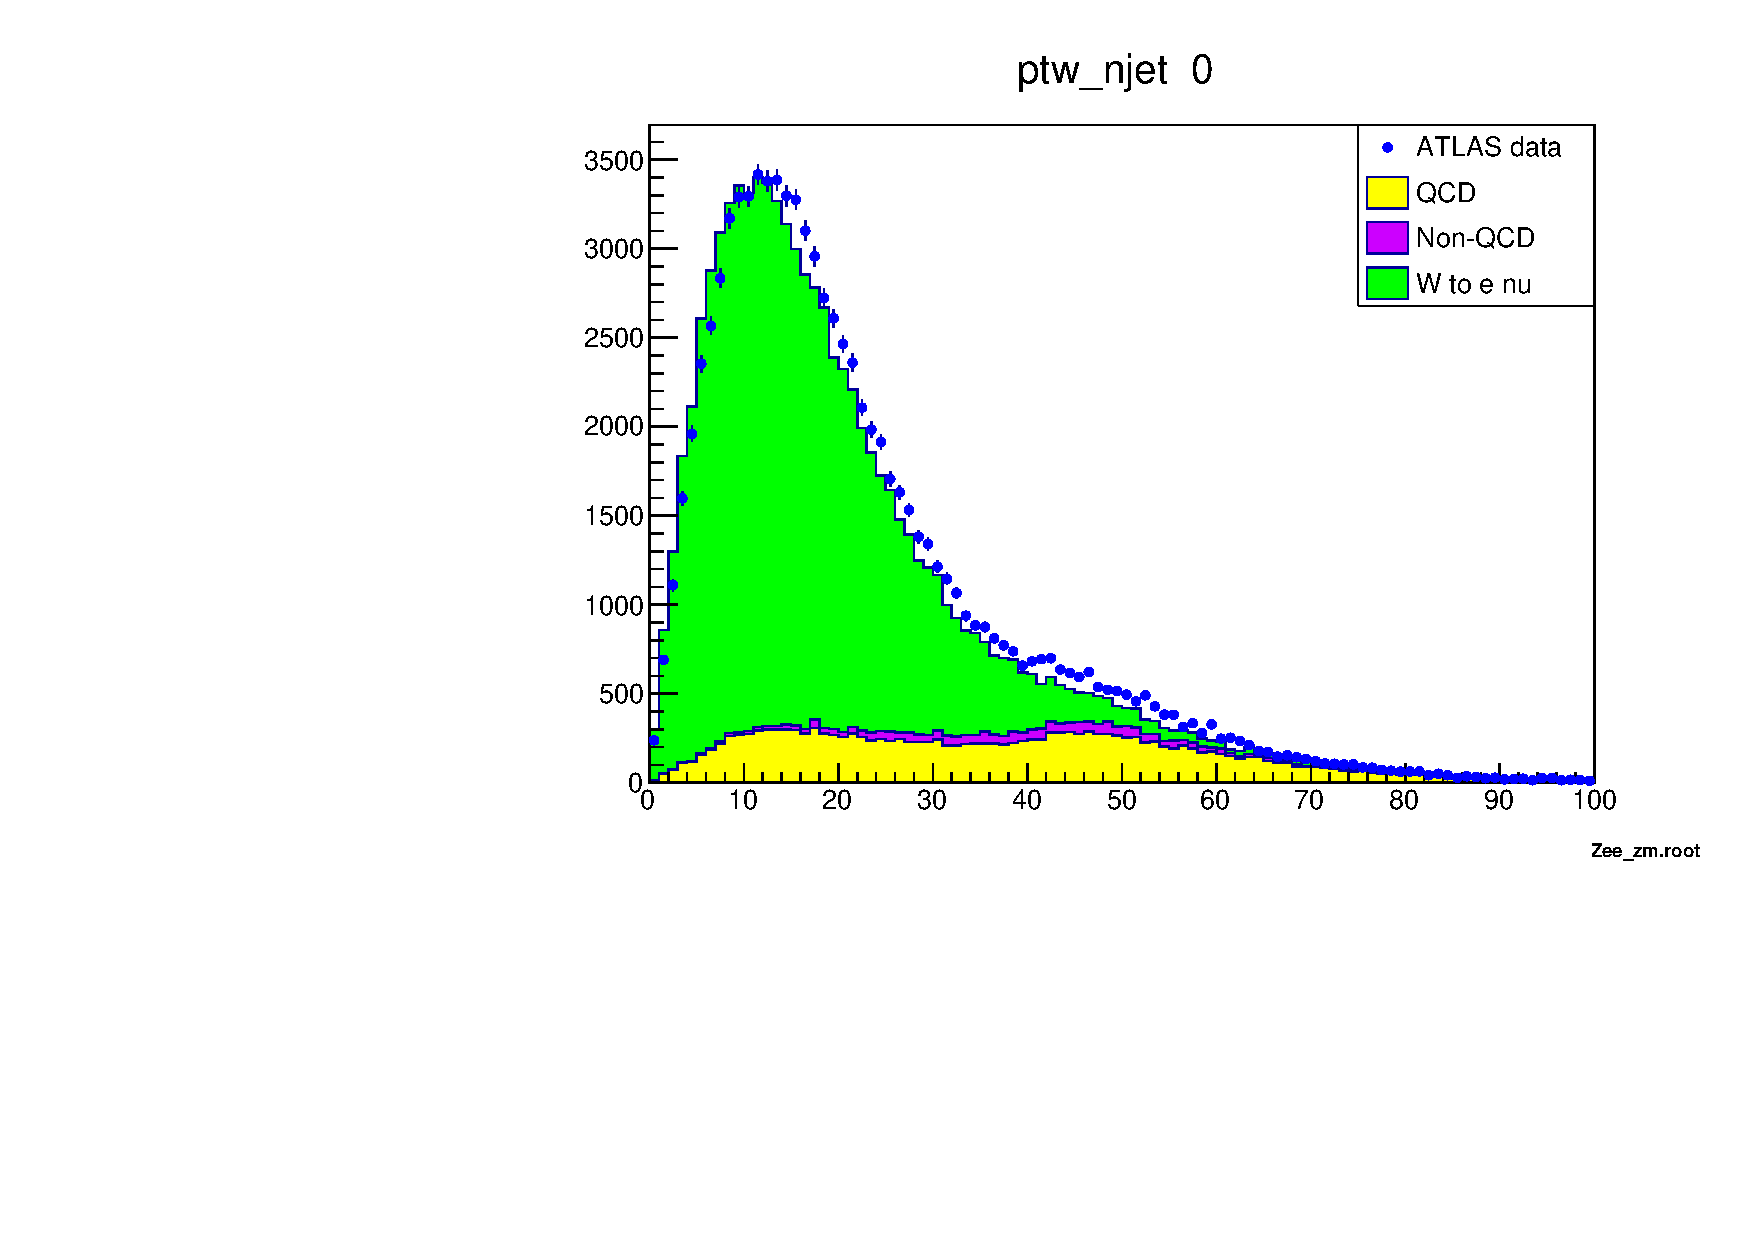
\includegraphics[width=\textwidth]{../W_mass/ptw_njet0.pdf}
            \subcaption{0 jets}
        \end{subfigure}
        \begin{subfigure}{0.5\textwidth}
            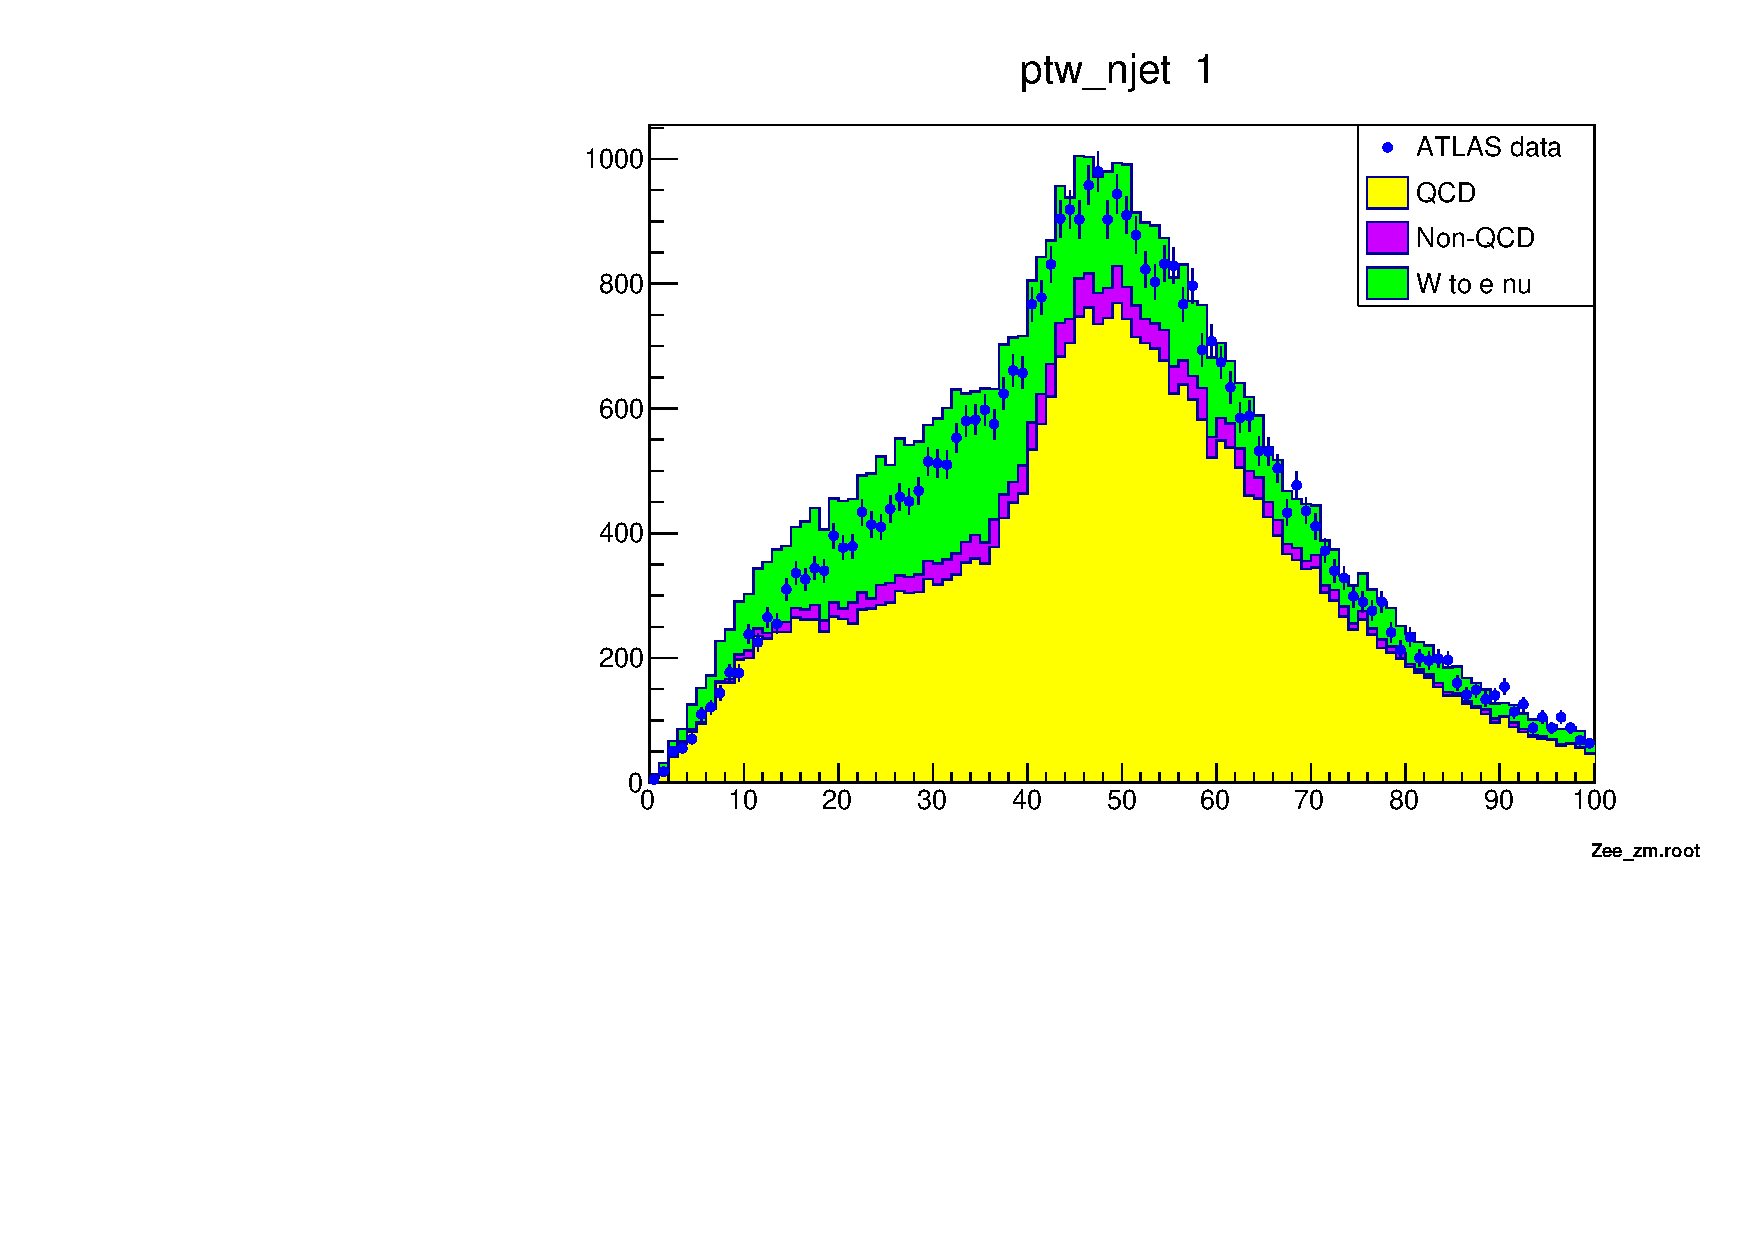
\includegraphics[width=\textwidth]{../W_mass/ptw_njet1.pdf}
            \subcaption{1 jet}
        \end{subfigure}
        \begin{subfigure}{0.5\textwidth}
            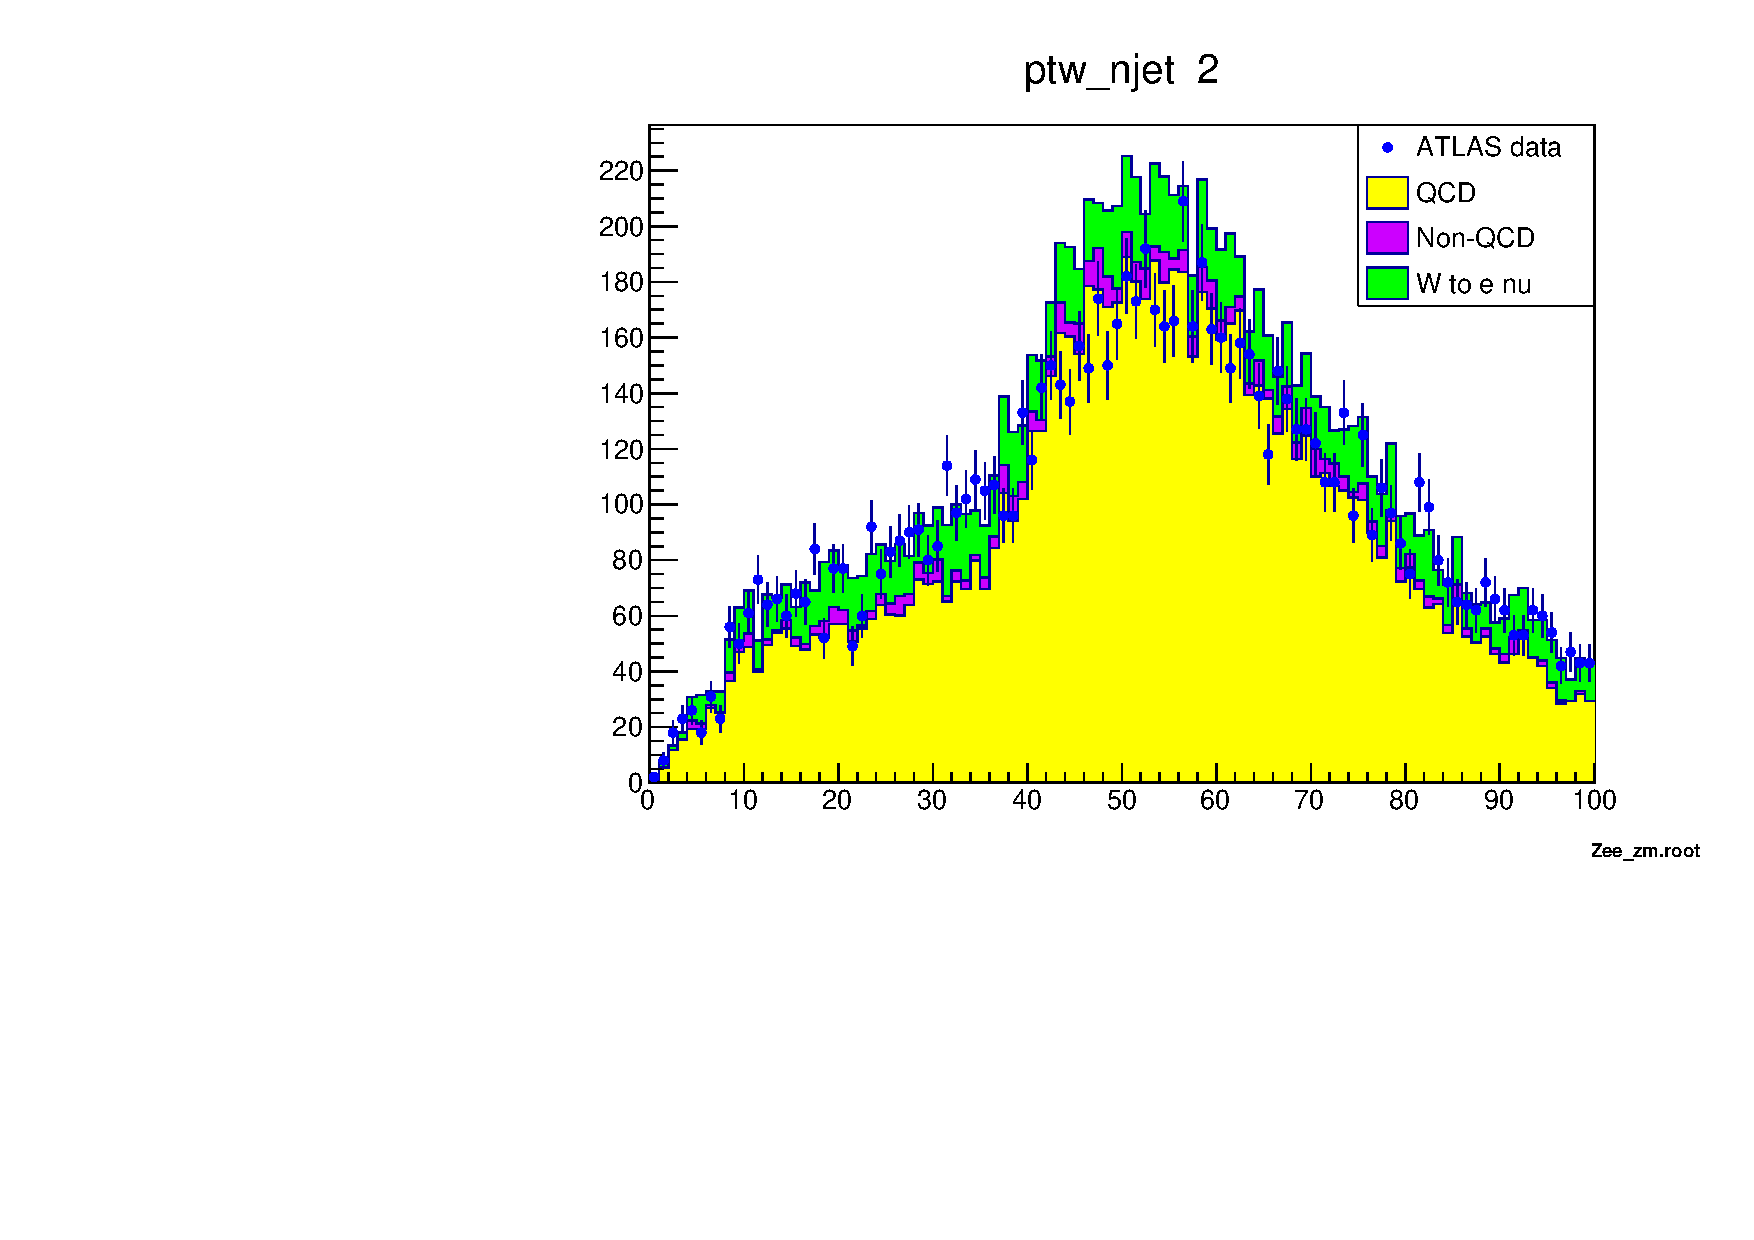
\includegraphics[width=\textwidth]{../W_mass/ptw_njet2.pdf}
            \subcaption{2 jets}
        \end{subfigure}
        \begin{subfigure}{0.5\textwidth}
            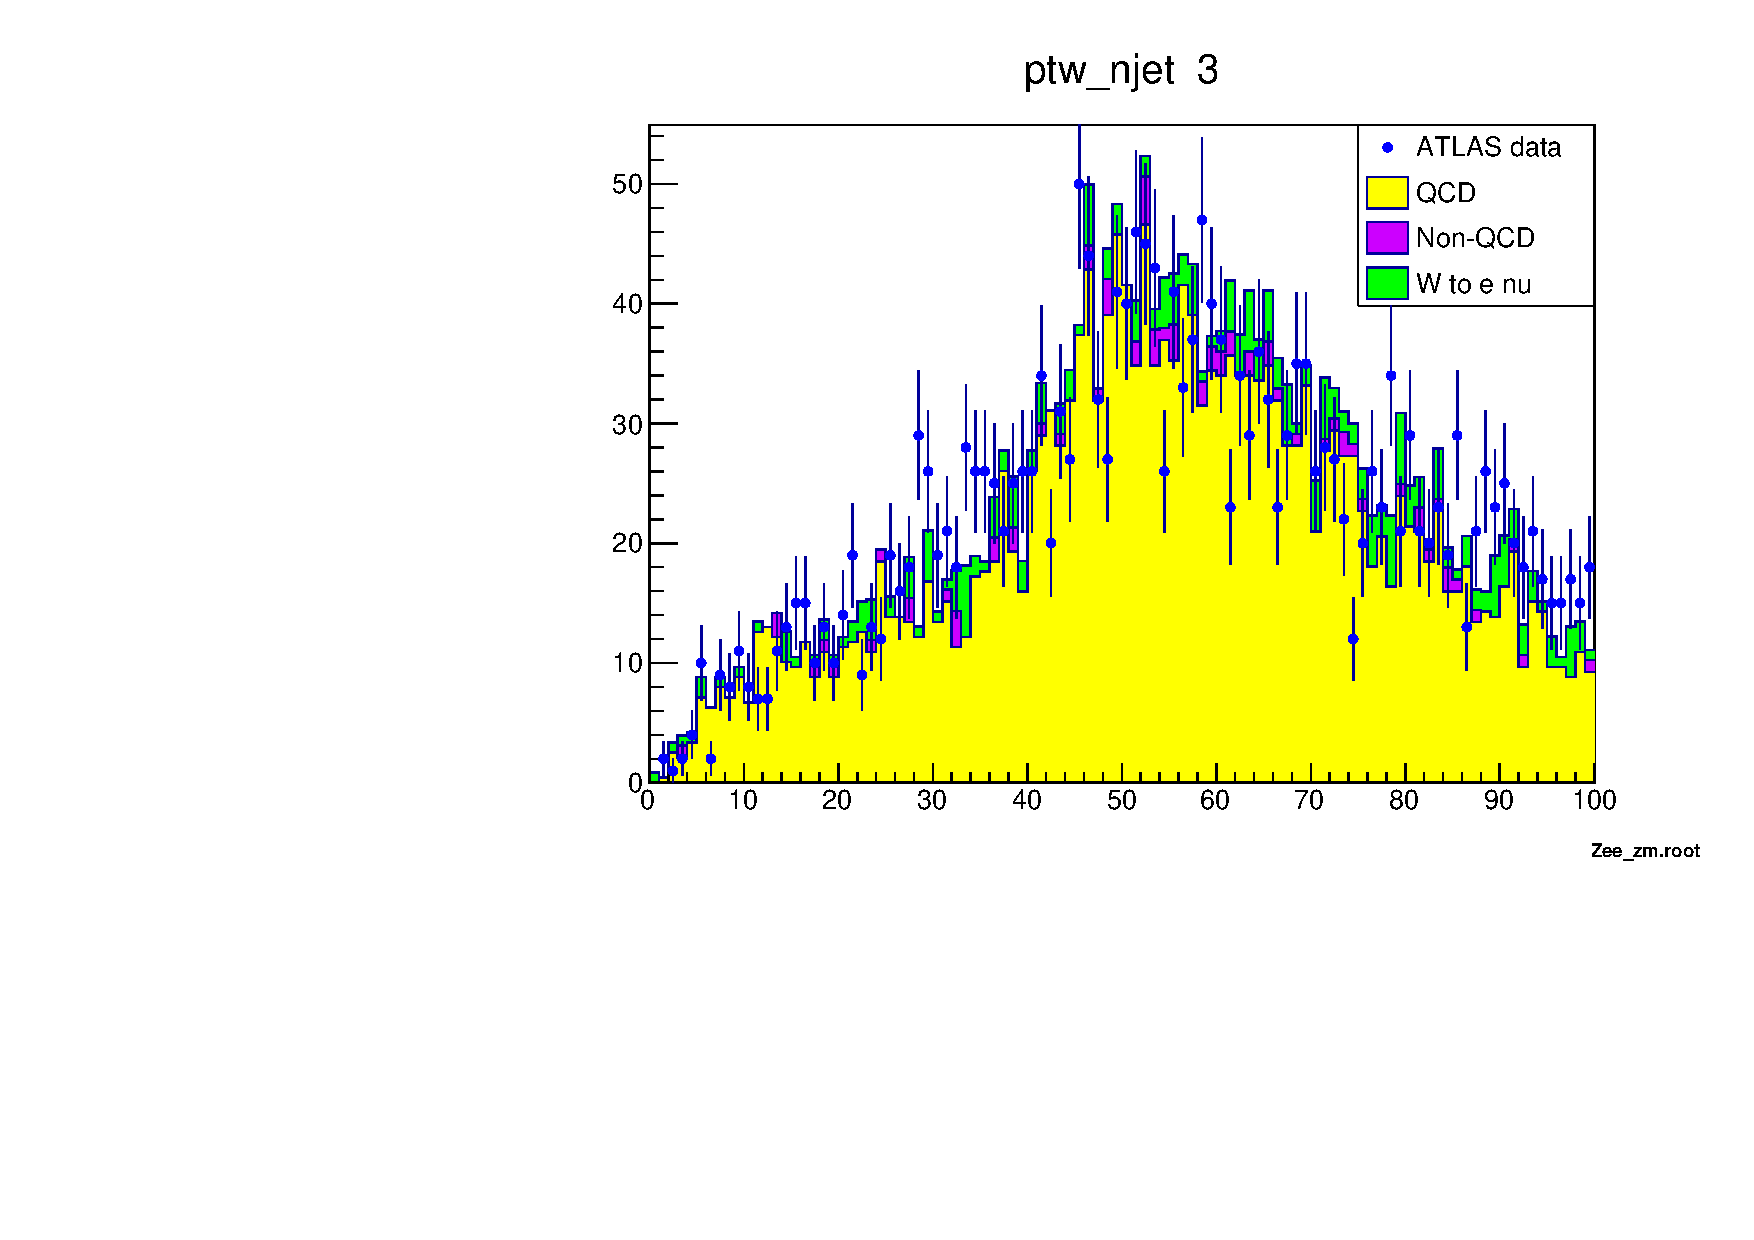
\includegraphics[width=\textwidth]{../W_mass/ptw_njet3.pdf}
            \subcaption{3 jets}
        \end{subfigure}
        \begin{subfigure}{0.5\textwidth}
            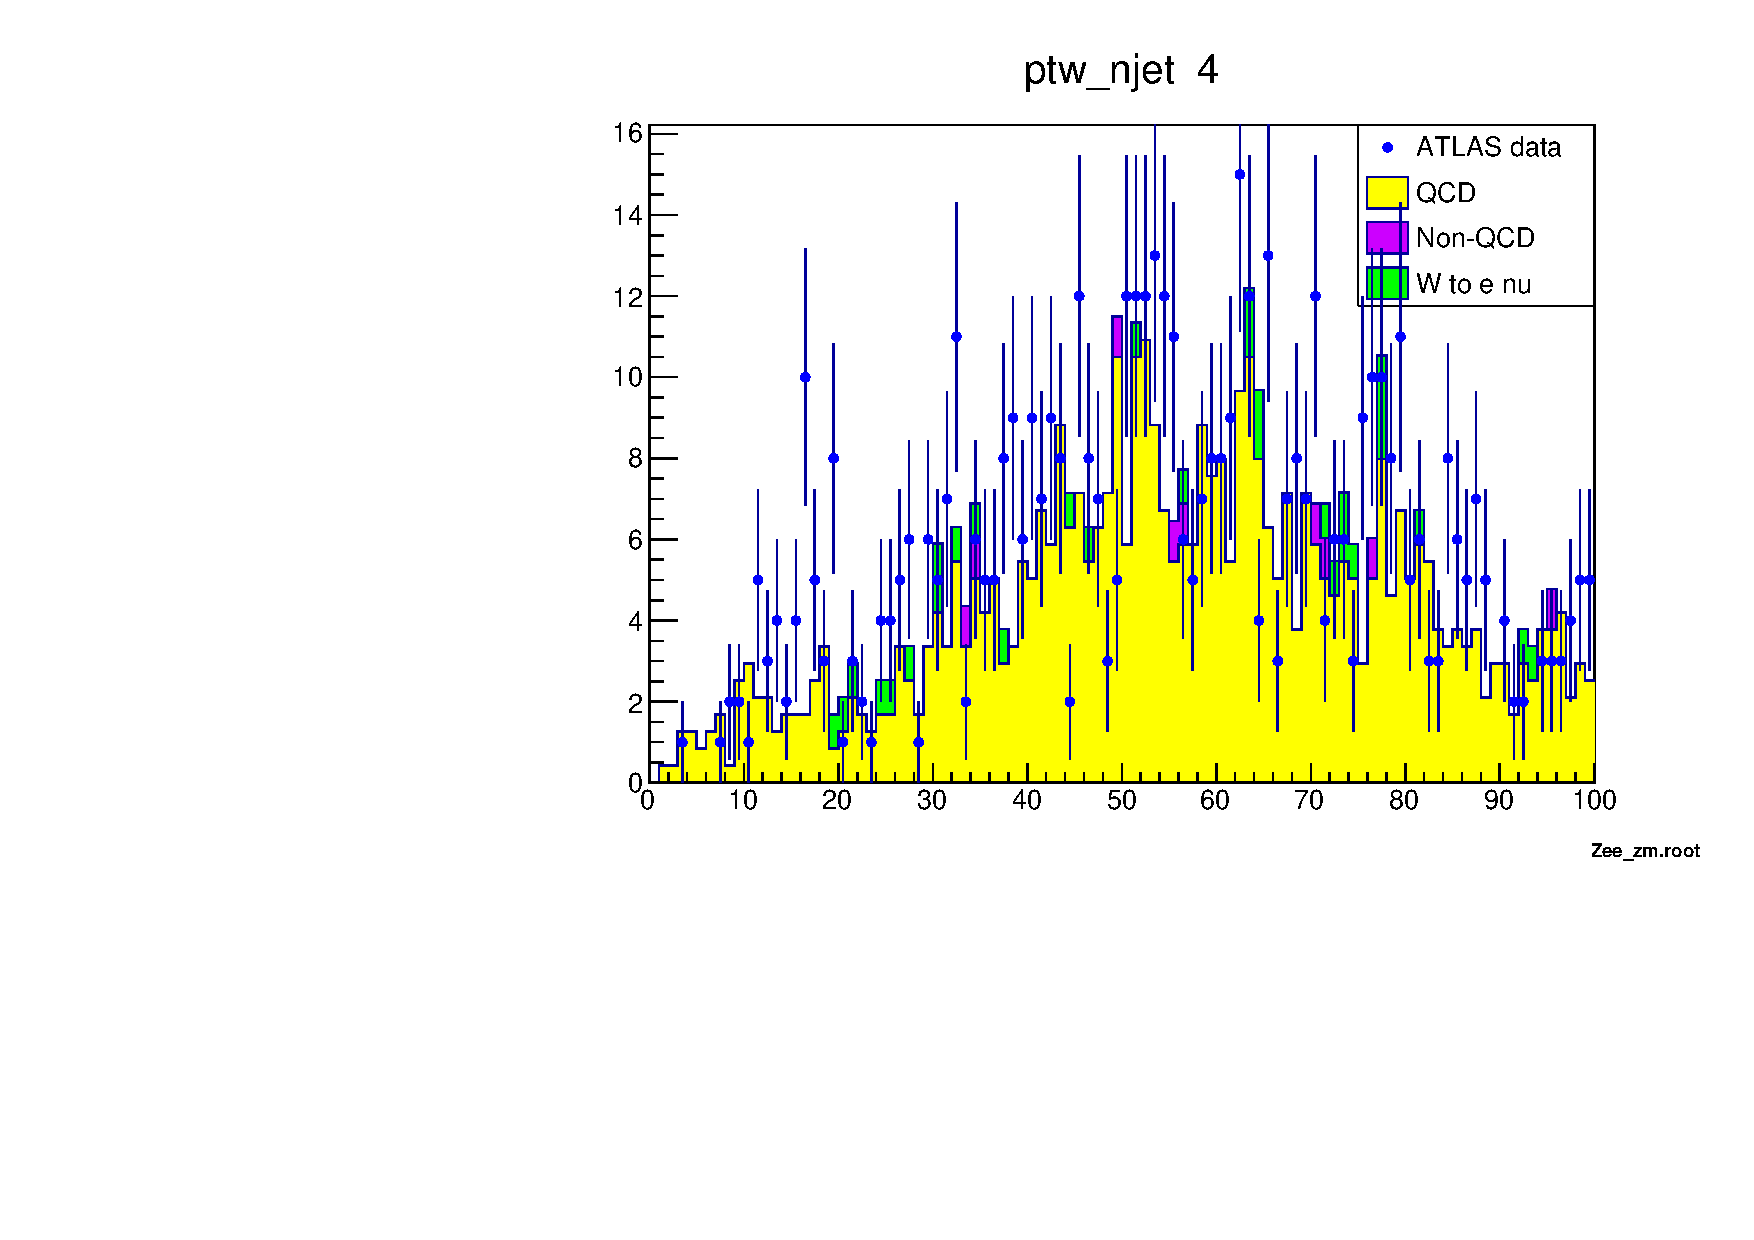
\includegraphics[width=\textwidth]{../W_mass/ptw_njet4.pdf}
            \subcaption{4 jets}
        \end{subfigure}
        \caption{\texttt{ptw} distributions for different number of jets measured in the events}
        \label{fig:ptw_jets}
    \end{figure}
    
\subsubsection{Final QCD scale factor}
    \label{sec:final_qcd}
    After examining the different kinematic variables, a final QCD scale factor has to be chosen.
    In order to do so, a region with high QCD background is chosen. For this we used to distribution of \texttt{ptw}, since the signal consists mostly of QCD background
    for energies larger than around 30 GeV, as can be seen in figure \ref{fig:qcd-final}. Therefore the cut
    \begin{align*}
        \texttt{ptw} > 30\,GeV
    \end{align*}
    is applied. To further increase the background, only events where the number of jets is larger than zero are taking into account, since we can see from
    figure \ref{fig:ptw_jets}, that the background to signal ratio increases for events with more than one jet. Therefore the cut 
    \begin{align*}
        \texttt{njet} > 0
    \end{align*}
    was also applied. When looking at the two remaining kinematic variables, \texttt{el\_pt} and \texttt{etmis} in figure \ref{fig:qcd-final}, it can be observed, that
    the for momenta lower than 30\,GeV, the background dominates the signal.
    Therefore the cuts 
    \begin{align*}
        \texttt{el\_pt} < 30\, GeV \\
        \texttt{etmis} < 30\, GeV
    \end{align*}
    were also applied. The resulting distribution for different QCD scale factors can be seen in figure \ref{fig:final_ptw}.
    The optimal value where the agreement between real and simulated data was identified by eye at $c_{QCD}=0.35$. The \texttt{ptw} distribution for that scale factor can 
    be seen in part (b) of figure \ref{fig:final_ptw}.
    To determine the error bounds of the QCD scale factor, the QCD scale factor was varied until the simulated and real data deviated visibly.
    The final QCD scale factor was then chosen as 
    \begin{align*}
        c_{QCD} = 0.35_{-0.05}^{+0.04} 
    \end{align*}
    Since this entire process was only done per eye, this result is highly subjective. However, in the following step, the background will be reduced as much as possible,
    therefore the QCD scale factor does not have a very large impact on the final result of $m_W$. 
    \begin{figure}
        \begin{subfigure}{0.5\textwidth}
            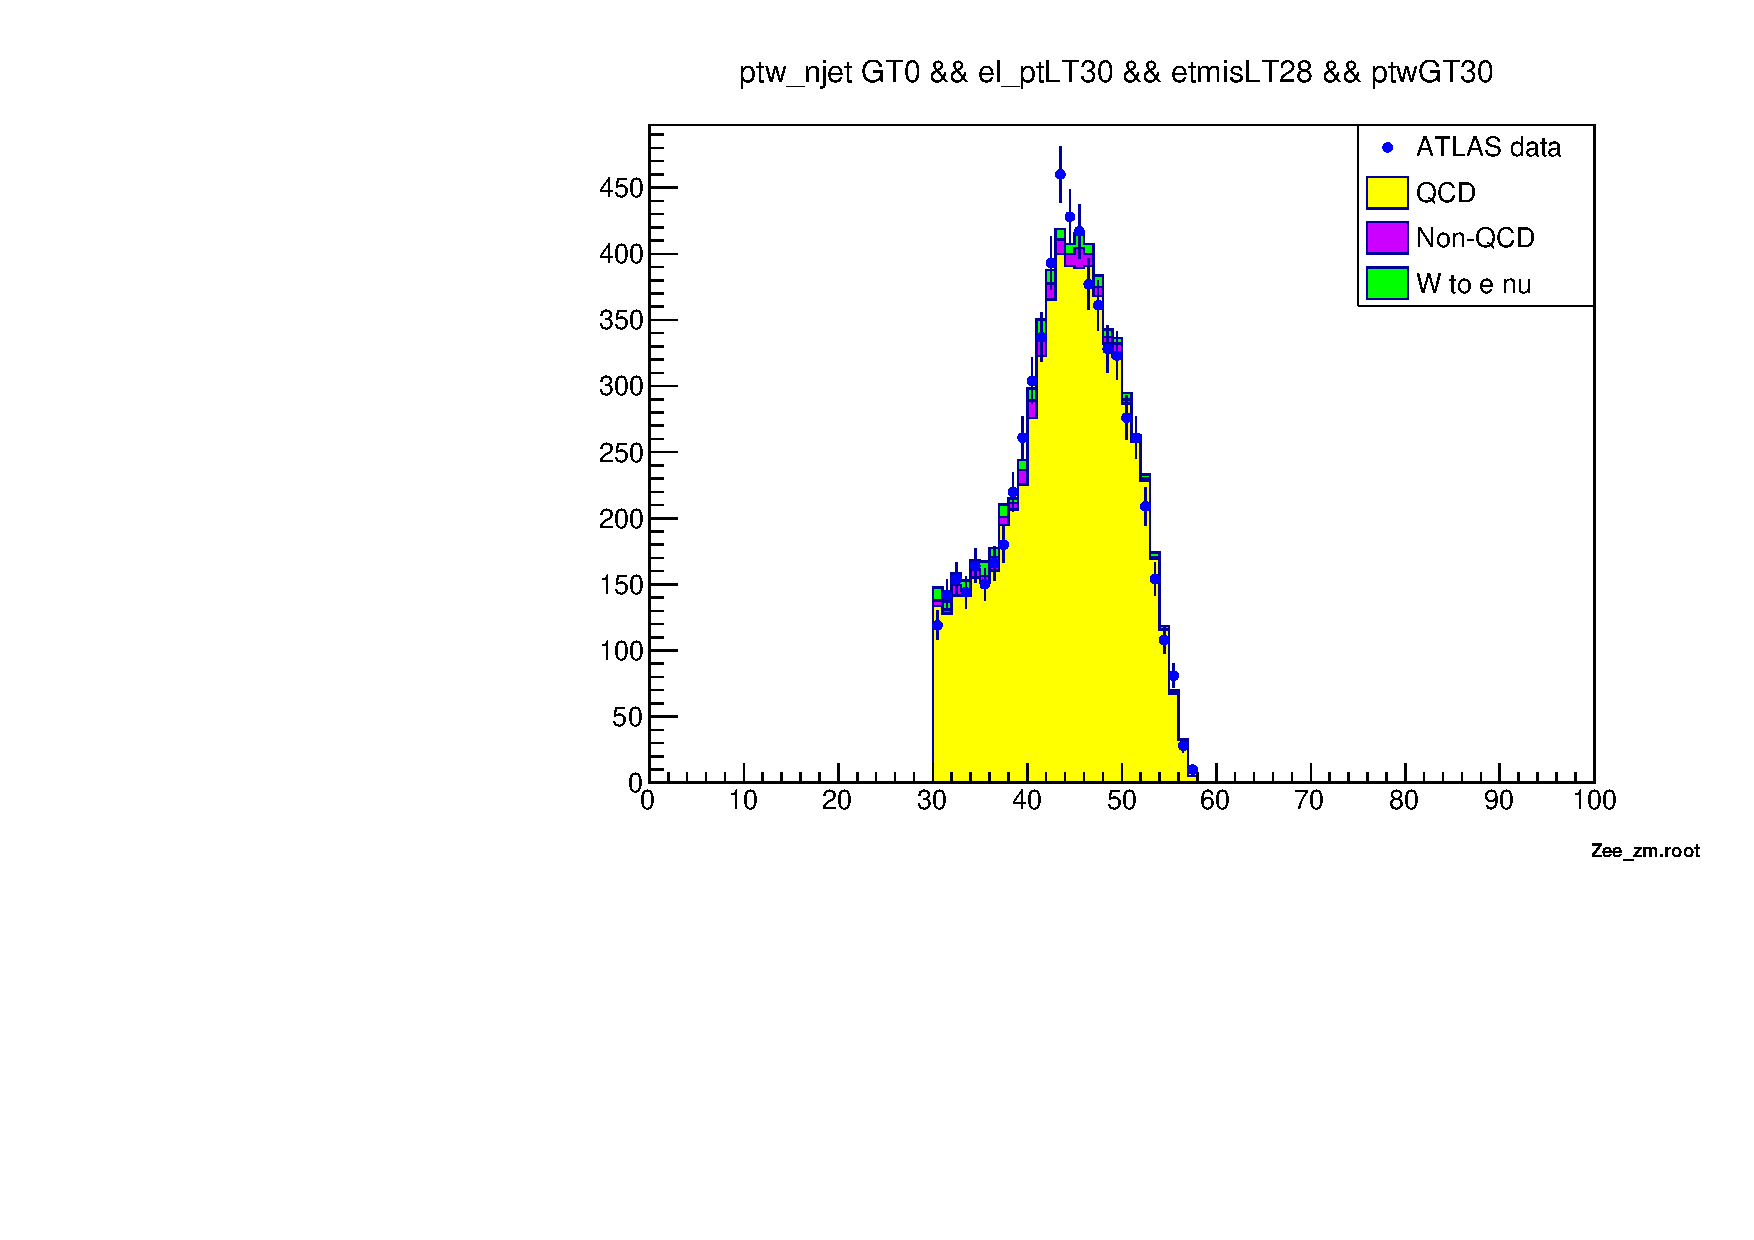
\includegraphics[width=\textwidth]{../W_mass/final_ptw_qcd0-33.pdf}
            \subcaption{QCD scale factor = 0.33}
        \end{subfigure}
        \begin{subfigure}{0.5\textwidth}
            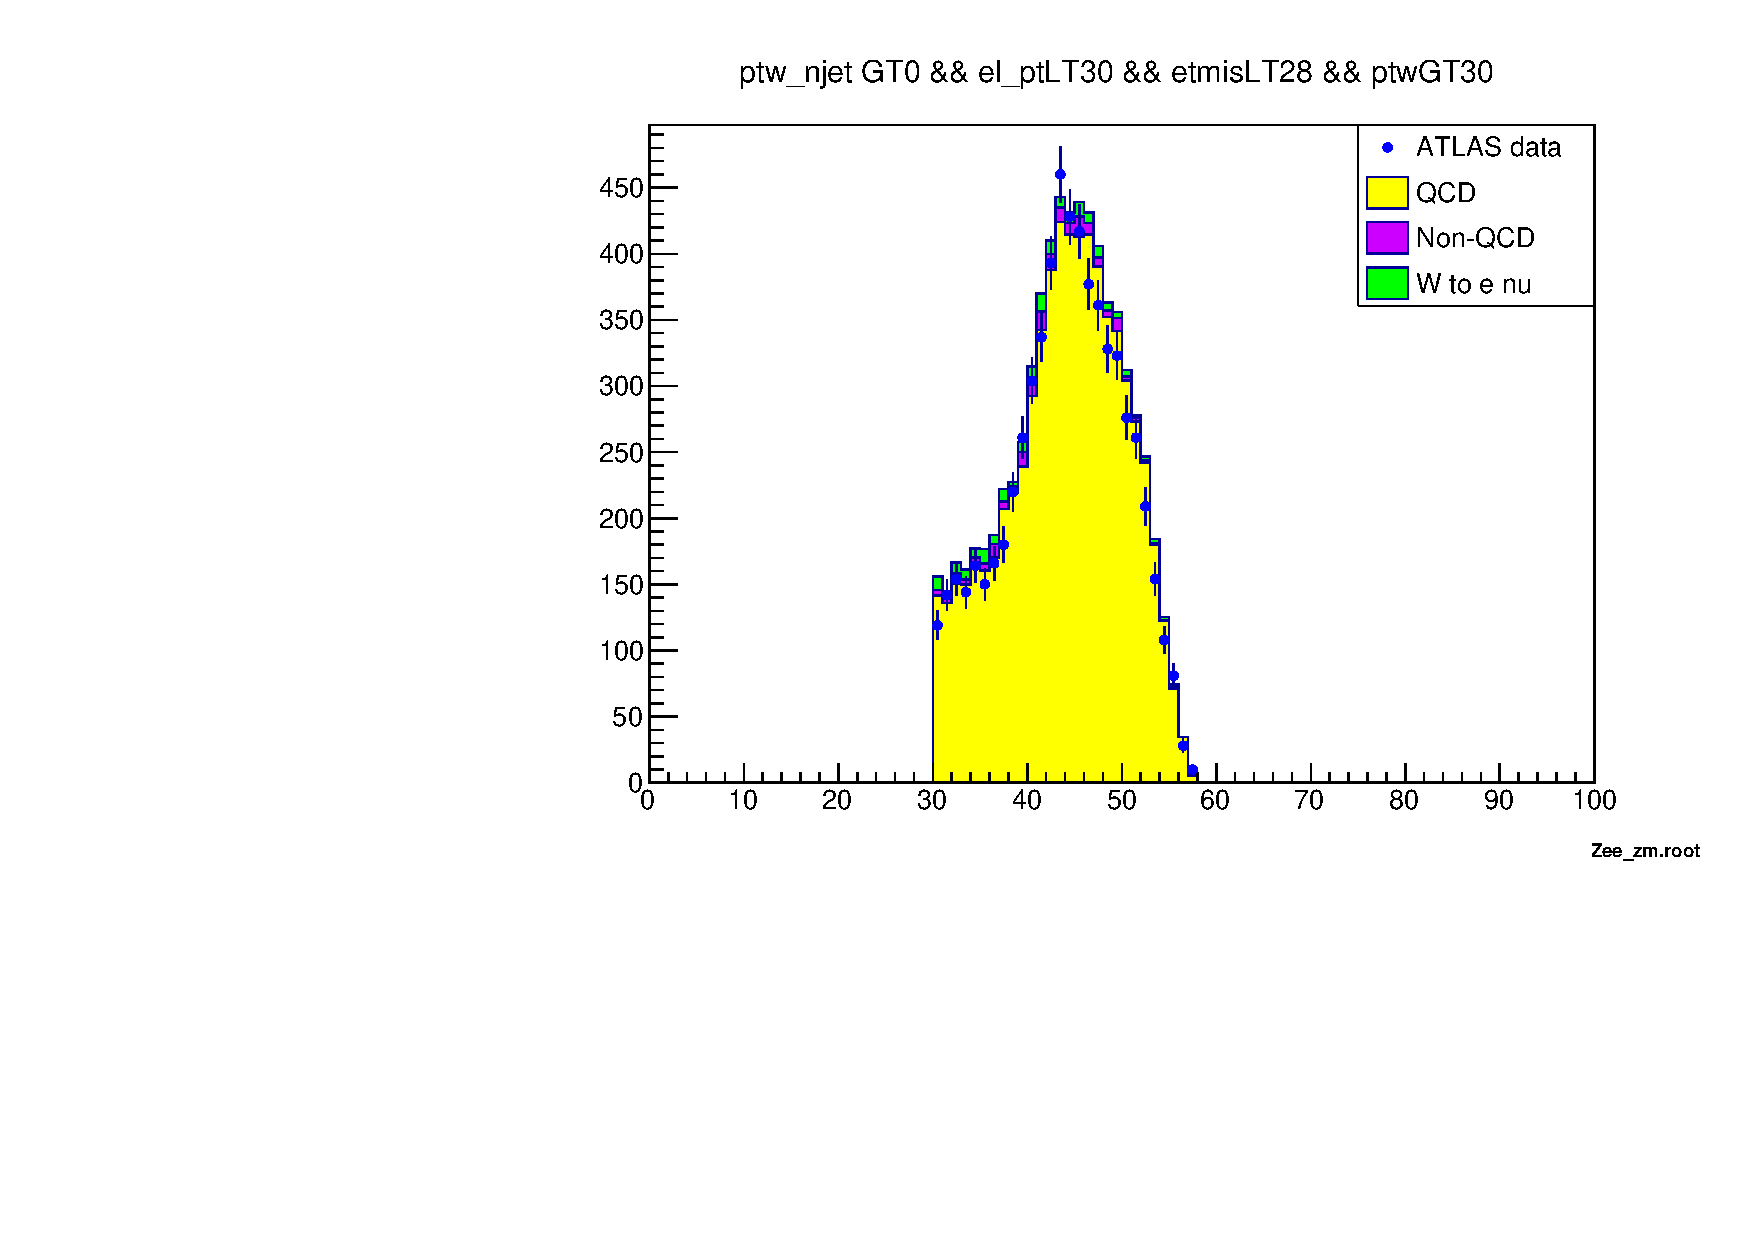
\includegraphics[width=\textwidth]{../W_mass/final_ptw_qcd0-35.pdf}
            \subcaption{QCD scale factor = 0.35}
        \end{subfigure}
        \begin{subfigure}{0.5\textwidth}
            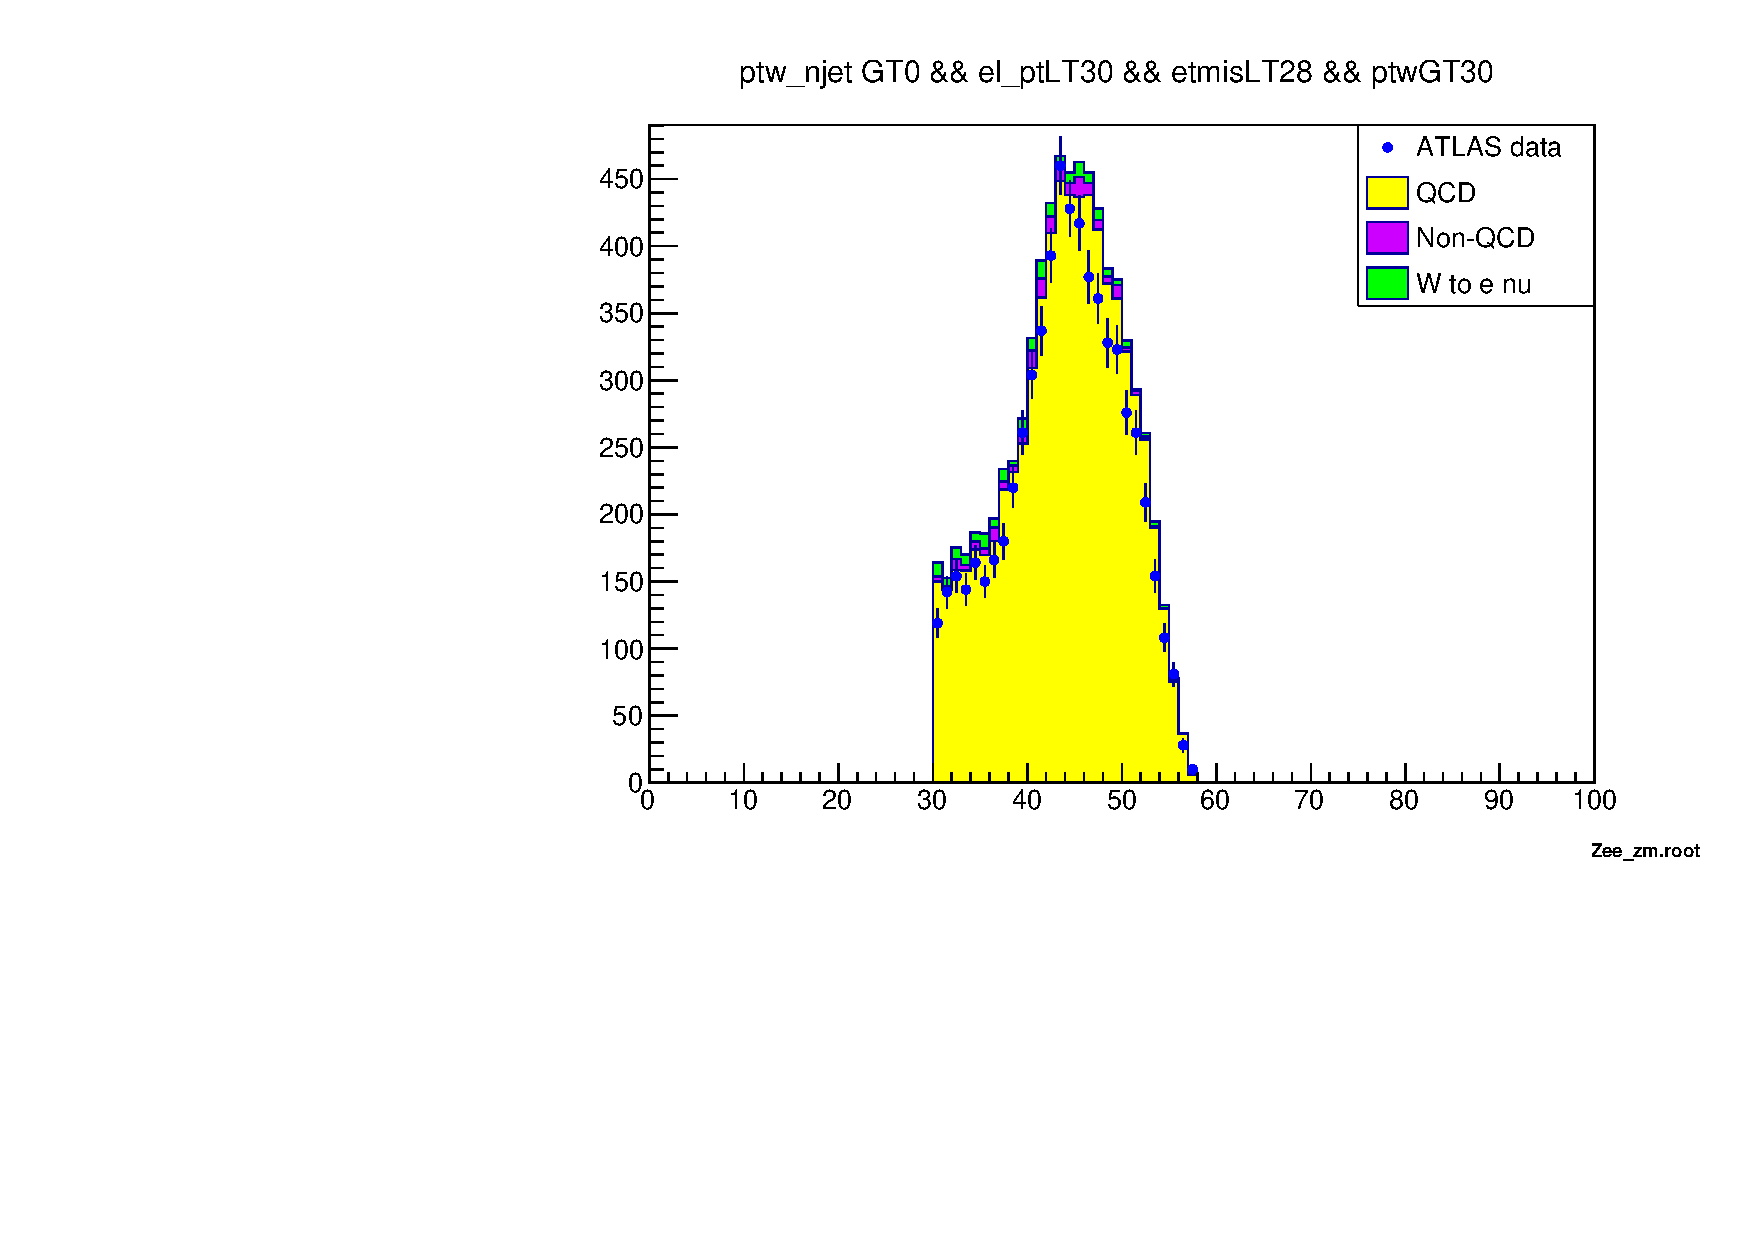
\includegraphics[width=\textwidth]{../W_mass/final_ptw_qcd0-37.pdf}
            \subcaption{QCD scale factor = 0.37}
        \end{subfigure}
        \caption{\texttt{ptw} distributions with the cuts \texttt{ptw} > 30\,GeV, \texttt{njet} > 0, \texttt{el\_pt} < 30\, GeV and \texttt{etmis} < 30\, GeV for different QCD
        scale factors}
        \label{fig:final_ptw}
    \end{figure}

\subsection{Cut selection}
    \label{sec:cut_seclection}
    In order to achieve the most accurate $m_W$ a cut selection has to be applied, so that the distribution of the \texttt{el\_pt}, which is used to calculate $m_W$,
    has the highest signal to background ratio. In order to choose the proper cut selections, the distributions of the kinematic variables in figures \ref{fig:qcd-final}
    and \ref{fig:ptw_jets} are examined again. The following cuts were chosen:\\
    \\
    Since there are no jets expected in $W \rightarrow e\nu$ events, which can be confirmed when looking at figure \ref{fig:ptw_jets} where the signal to  
    background ratio decreases significantly as the number of jets increases, the cut \texttt{njet == 0} is applied.\\
    \\
    Since there is a neutrino present in the $W$ decay, missing transverse momentum/energy $\slashed{E}_T$ is expected in the events.
    When looking at the \texttt{etmis} distribution in figure \ref{fig:qcd1}, the background is largest for small $\slashed{E}_T$. After some trial and error, the cut
    \texttt{etmis} > 33\,Gev is chosen.\\
    \\
    It is expected, that the $W$ boson itself does not have a large transverse momentum, which can be confirmed when looking at the \texttt{ptw} distribution
    in figure \ref{fig:qcd1}. Therefore events with large \texttt{ptw} are cut off. The final cut was chosen as \texttt{ptw} < 35\,GeV.\\
    \\
    So the final cut 
    \begin{align*}
        \texttt{njet == 0 \&\& etmis > 33 \&\& ptw < 35}
    \end{align*}
    is applied to the \texttt{el\_pt} distribution. The distribution of \texttt{el\_pt} with the cuts applied can be seen in figure \ref{fig:el_pt_cuts}
    \begin{figure}
        \centering
        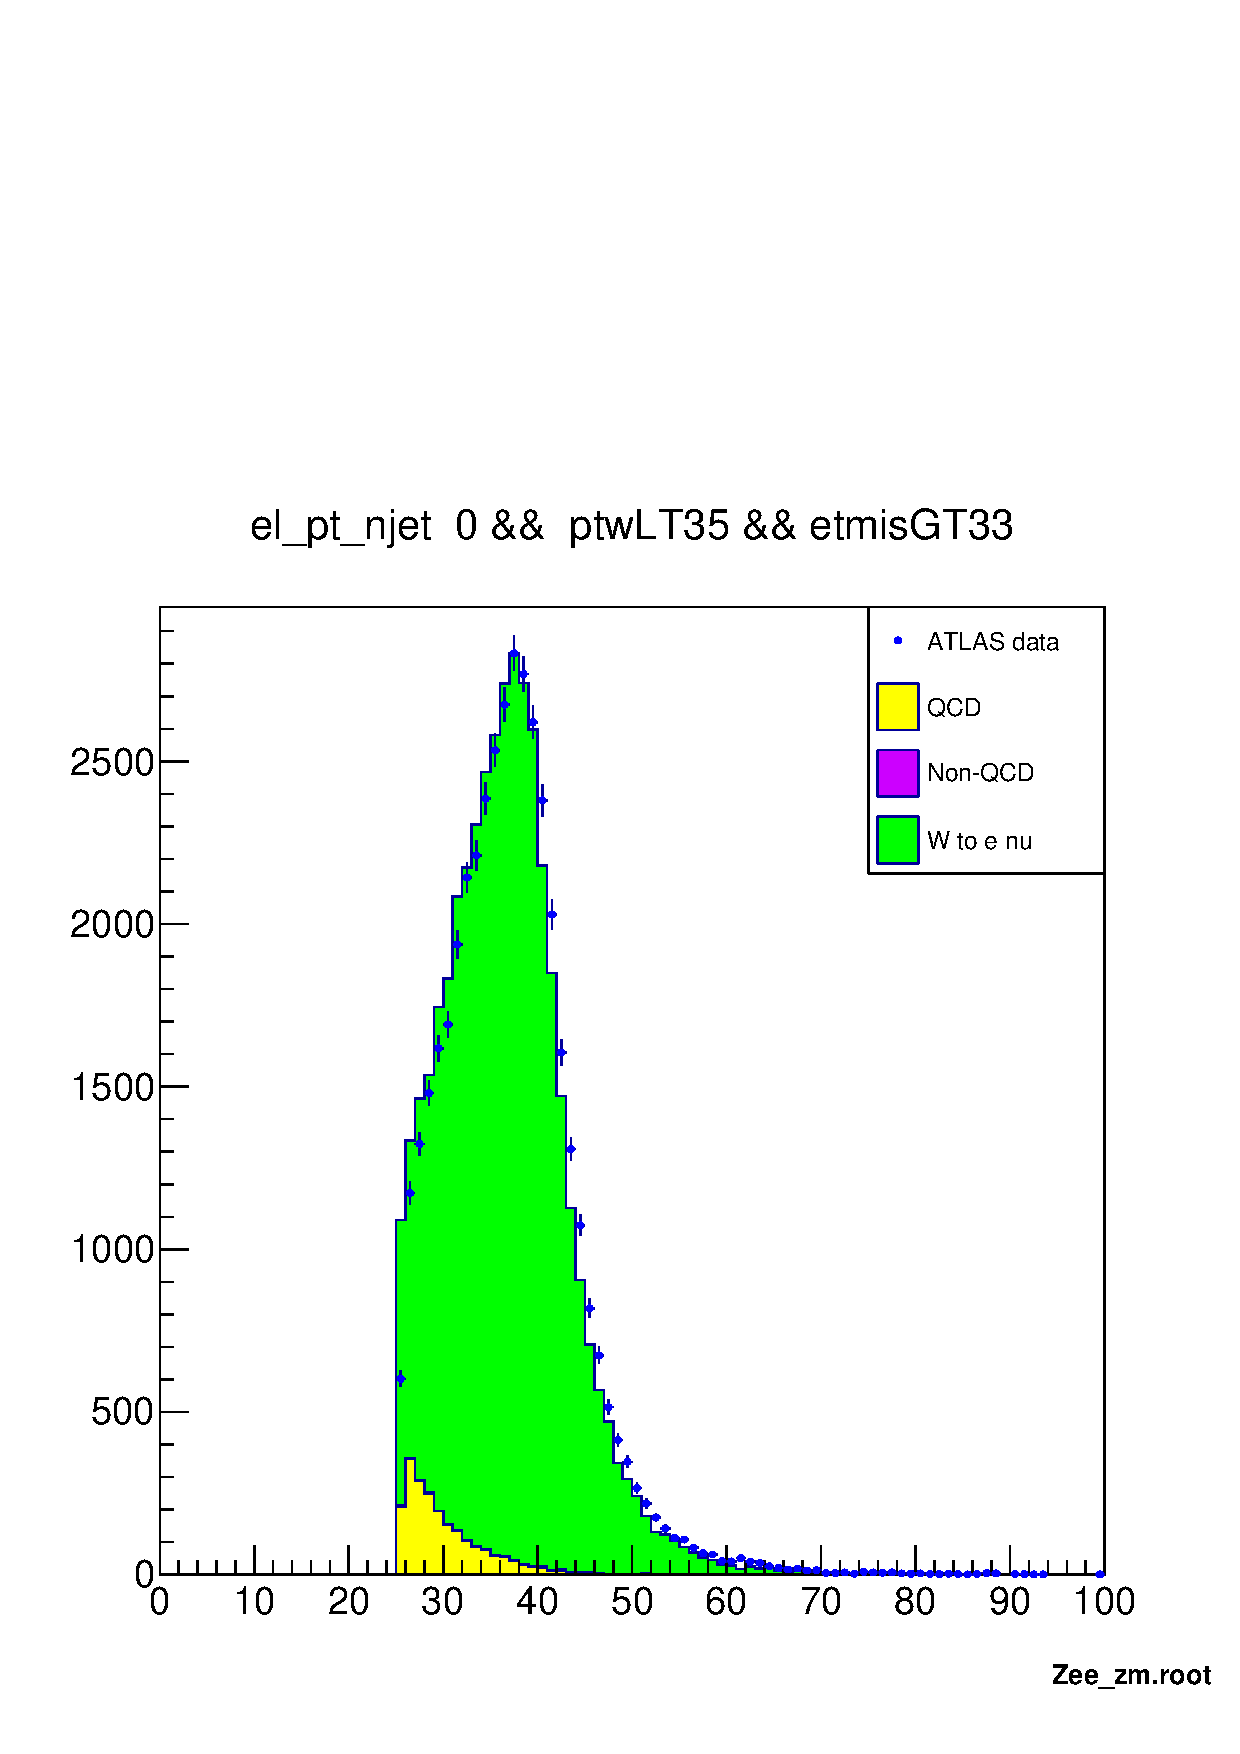
\includegraphics[width=0.6\textwidth]{../W_mass/el_pt_final_cut_selection.pdf}
        \caption{Electron transverse momentum \texttt{el\_pt} with the cuts \texttt{njet == 0 \&\& etmis > 33 \&\& ptw < 35} applied.}
        \label{fig:el_pt_cuts}
    \end{figure}
    When comparing the \texttt{el\_pt} distribution with the cuts and the final QCD scale factor applied, to the \texttt{el\_pt} distribution in figure \ref{fig:qcd1},
    the agreement between simulated and real data is increased whilst the background is decreased significantly. Therefore the applied cuts as well as the QCD scale factor
    seem to be a decent choice.

\section{$W$ boson mass}
    With the QCD scale factor set, and the cuts to the different kinematic regions applied, the mass of the $W$ boson can now be calculated.
    This is done with the Jacobi-Peak in the electron transverse momentum distribution \texttt{el\_pt}. However, the peak is not very clear, as can be seen in figure
    \ref{fig:el_pt_cuts}. This is amongst other things mostly due to decay width of the $W$ boson and the limited resolution of the detector. 
    Therefore a different approach, making use of the half maximum point of the distribution is chosen. The effects of the detector resolution and the decay width 
    of the $W$ boson on the electron transverse momentum distribution are assumed to be symmetric \cite{atlaslabmanual}. Therefore even though the peak is not clear in the distribution,
    the half maximum point should be not change. This assumption is used to extract the $W$ boson mass using the gauge curves.

\subsection{Gauge curves}
    \label{sec:gauge_curves}
    In order to extract the mass of the $W$ boson from the electron transverse momentum distribution, using the half maximum point, the cuts and the QCD scale factor 
    discussed in section \ref{sec:qcd_factor/variables} are applied to the real ATLAS data and simulated $W \rightarrow e\nu$ data sets for different $m_W$.
    This is also done for one set of $Z^0 \rightarrow e^+e^-$ data to use as a check wether the fits work in general or just for the $W$ by coincidence.   
    For each of these distributions, the half maximum point is determined using a fit. \cite{atlaslabmanual}
    The distributions with applied cuts and fits, can be seen in figure \ref{fig:gauge_curve_cuts1}.
    Then the $W$ masses of the simulated data sets are plotted against the extracted half maximum of the electron transverse momentum $p_T^h$ in a so called gauge curve.
    This can be seen in figure \ref{fig:gauge1}
    \begin{figure}
        \centering
        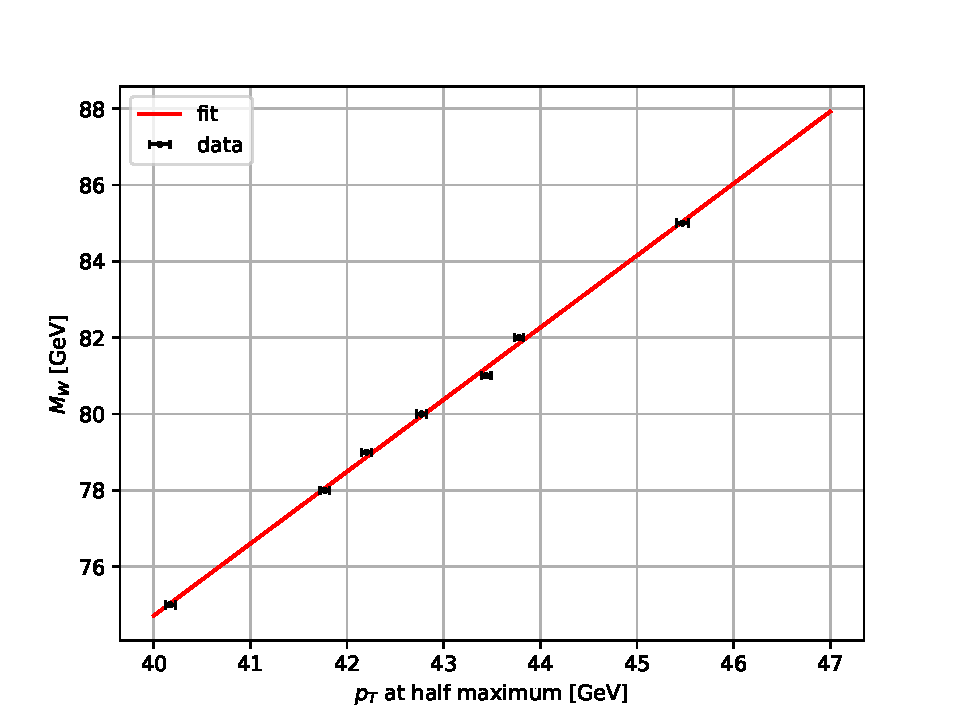
\includegraphics[width=0.7\textwidth]{../W_mass/gauge1.pdf}
        \caption{$W$ boson masses from the different data sets plotted against the half maximum points of the Jacobi peak in the electron transverse momentum distribution.}
        \label{fig:gauge1}
    \end{figure}
    The fit used for the gauge curves was done with the function
    \begin{equation}
        \label{eqn:gauge}
        M_w(p_T) = a \cdot p_T^h + b
    \end{equation}
    In order to obtain the mass of the $W$ boson, the electron transverse momentum at half maximum of the actual ATLAS data has to be inserted into equation \ref{eqn:gauge}.
    For the first set of fits in figure \ref{fig:gauge_curve_cuts1} and the resulting gauge curve in figure \ref{fig:gauge1}. The fit parameters were to determined to 
    \begin{align*}
        a = 1.886 \pm 0.033 \ \ \mathrm{and} \ \ b = (-0.732 \pm 1.420)\,\mathrm{GeV}  \\
    \end{align*}
    The error of parameter $b$ is large compared to the value of $b$. Since in theory $b$ is expected to be zero, and the fit is done in a range, that is not near zero,
    the fact that $b$ has such a large error is of course unwanted, but not unexpected. The value of parameter $a$ is somewhat expected as well.
    Due to the Jacobi peak being located at half the $W$ boson mass, a slope of 2 is expected in theory. Therefore a value of $a=1.886$ is not far away from that.
    In order to determine the error of the real $W$ boson mass, the errors of $p_T^h$, the errors fit parameters as well as their covariance have to be taken into consideration.
    Using gaussian error propagation, the error of the final $W$ boson mass can be calculated using 
    \begin{equation}
        \label{eqn:gague_err}
        \sigma^2_{M_W} = \left( \frac{\partial M_W}{\partial a} \cdot \sigma_a \right)^2 + \left( \frac{\partial M_W}{\partial b} \cdot \sigma_b \right)^2 
        + 2 \cdot \frac{\partial M_W}{\partial a} \cdot \frac{\partial M_W}{\partial b} \cdot \sigma_{ab} 
        + \left( \frac{\partial M_W}{\partial p_T^{\mu}} \cdot \sigma_{p_T^{\mu}} \right)^2.
    \end{equation}
    Here $\sigma_{ab}$ is the covariance between the fit parameters. It is assumed that $p_T^h$ is not correlated with the errors of $a$ and $b$.
    Using the fit which can be seen in figure \ref{fig:gauge1} and equations \ref{eqn:gauge} and \ref{eqn:gague_err}, the mass of the $W$ boson is calculated
    to $m_W = (81.037 \pm 0.431)$\,GeV.
    The same thing can be done for the $Z^0$ mass, which is calculated to $m_{Z^0} = (91.638 \pm 0.316)$\,GeV.
    

\subsection{Adjusting cuts and fit range}
    \label{sec:adjusting}
    Since the $W$ boson mass calculated in section \label{sec:gauge_curves} deviates significantly from the literature value $m_W^{lit} = (80.3692 \pm 0.0133)$\,GeV \cite{PDG2024}
    the fits to the Jacobi-peaks still needs to be improved. The possible parameters which can be adjusted is the fit range of the fit applied to the Jacobi-peak 
    as well as the readjusting the cuts on the \texttt{el\_pt} distributions.
    Starting with the fit range, the procedure of fitting the Jacobi-peak, creating the gauge curve and extracting the mass of the $W$ and the $Z^0$ boson, is done 
    for a set off different ranges. A list of the ranges and the corresponding $W$ and $Z^0$ masses can be seen in table \ref{tab:ranges}
    \begin{table}[H]
        \centering
        \begin{tabular}{ccc}
            \toprule
            fit range / GeV & $m_W$ / GeV & $m_{Z^0}$ / Gev \\
            \midrule
            30 to 55    & $81.037 \pm 0.431$  &  $91.638 \pm 0.316$ \\
            27 to 55    & $81.068 \pm 0.428$  &  $91.816 \pm 0.321$ \\
            32 to 55    & $80.931 \pm 0.372$  &  $91.782 \pm 0.374$ \\
            32 to 53    & $80.914 \pm 0.451$  &  $91.689 \pm 0.412$ \\
            32 to 50    & $80.884 \pm 0.503$  &  $91.507 \pm 0.377$ \\
            32 to 60    & $80.952 \pm 0.327$  &  $91.958 \pm 0.428$ \\
            \bottomrule
        \end{tabular}
        \caption{$w$ and $Z^0$ boson masses for different fit ranges to to Jacobi-peak fit}
        \label{tab:ranges}
    \end{table}
    Since the calculated value of $m_W$ was closest to the literature value for the range 32 to 55\,GeV, this range is chosen for all future fits.\\
    Another way to further increase the quality of the fit is to readjust the cuts applied to the transverse electron momentum distribution.
    After some initial tries, adjusting the \texttt{ptw} did not seem to have any effect on the fit, and cutting on \texttt{el\_pt} has the same effect as the the fit range,
    since the fit range already regulates which values of \text{el\_pt} are taken into the fit. Therefore the remaining cut is the one on $\slashed{E}_T$, meaning that the cut 
    \texttt{etmis > 33} which we chose in section \ref{sec:cut_seclection} is adjusted to achieve the best result for the $W$ boson mass.
    Again the same procedure which was done for the different fit ranges is repeated for different cuts in \texttt{etmis}. The cuts, and the corresponding $W$ and $Z^0$ masses
    can be seen in table \ref{tab:etmis}
    \begin{table}[H]
        \centering
        \begin{tabular}{ccc}
            \toprule
            cut selection / GeV & $m_W$ / GeV & $m_{Z^0}$ / Gev \\
            \midrule
            \texttt{etmis > 35}     & $80.899 \pm 0.346$  &  $91.339 \pm 0.378$ \\
            \texttt{etmis > 20}     & $80.252 \pm 0.256$  &  $91.502 \pm 0.314$ \\
            \texttt{etmis > 25}     & $80.431 \pm 0.278$  &  $91.457 \pm 0.345$ \\
            \texttt{etmis > 24}     & $80.391 \pm 0.215$  &  $91.441 \pm 0.281$ \\
            \bottomrule
        \end{tabular}
        \caption{$w$ and $Z^0$ boson masses for different cuts on the \texttt{etmis}.}
        \label{tab:etmis}
    \end{table}
    The final entry in table \ref{tab:etmis} is the cut which gave the best result, meaning that $m_W$ is closest to the literature value.
    To summarize, the final chosen parameters for the calculation of the $W$ boson mass, are the QCD scale factor $c_{QCD} = 0.35_{-0.05}^{+0.04}$ (where $c=0.35$ was used)
    and the cuts \texttt{njet == 0 \&\& ptw < 35 \&\& etmis > 24} were used to obtain a $W$ and $Z^0$ boson mass of 
    \begin{align*}
        m_W  & = (80.391 \pm 0.215)\,\mathrm{GeV}  \\
        m_{Z^0} & = (91.441 \pm 0.281)\,\mathrm{GeV} \\
    \end{align*}
    The fits to the Jacobi-peaks for the final cut selection can be seen in figure \ref{fig:Jacobi-final}, and the gauge curve can be seen in figure \ref{fig:gauge_final}.
    The fit parameters from the gauge curve fit are $a=1.876 \pm 0.034$ and $b = (-0.241 \pm 1.453)$\,GeV.

\section{Systematic uncertainties}
    \label{sec:uncertainties}
    The uncertainty given for the mass of the $W$ boson in section \ref{sec:adjusting} are entirely statistical. However, systematic uncertainties have to be taken into 
    account as well. There are many sources of systematic uncertainties in the entire process to get the mass of the $W$ boson. The ones which can be evaluated within 
    our means are the calibration of the electron energy, the QCD scale factor, the fit range as well as the cut selection.

\subsection{Calibration uncertainty}
    The systematic uncertainty due to the electron calibration can not be calculated. In order to so, the entire process of finding the mass of the $W$ boson would need
    to be repeated for different calibrations, to get an understanding for the impact the calibration has on the final result. This would be beyond the scope of this 
    experiment. Therefore the uncertainty from the calibration of the electron energy can only be estimated. In order to do this, the largest uncertainty of the calculated
    $Z^0$ masses is used as uncertainty for the $W$ boson as well. This is not a very accurate way to determine this of uncertainty, it is however not likely, that the 
    $W$ boson uncertainty due to the calibration has a much larger value. Therefore the systematic uncertainty due to the calibration is chosen as $\pm0.05$\,GeV.

\subsection{QCD scale factor uncertainty}
    The QCD scale factor has an impact on the $W$ boson mass, since the background is not fully excluded in the Jacobi-peaks which are used to get $p_T^h$.
    This can be seen in figure \ref{fig:el_pt_cuts}. The background is small compared to the data, but not negligible. 
    Therefore in order to estimate the systematic uncertainty from the QCD scale factor, the analysis would again have to be repeated for different QCD scale factors.
    Since we were short on time, we were unable to repeat the analysis for different QCD scale factors. So the systematic uncertainty has to be estimated.
    When looking at figure \ref{fig:el_pt_cuts}, as mentioned before the QCD background is not negligible. It is however not very large. And the agreement between simulated
    and real ATLAS data is already quite good. Therefore the effect of the QCD scale factor on the analysis is most likely small even compared to the uncertainty from 
    the calibration. But since this cannot confirm be confirmed, the systematic uncertainty from the QCD scale factor is estimated to $\pm0.025$\,GeV. It is most likely smaller 
    than that, however since it cannot be confirmed a larger value is chosen to not underestimate the uncertainty.

\subsection{Fit range uncertainty}
    Another parameter which was used to optimize the fit was the range. The fit range was adjusted in section \ref{sec:adjusting} until the range which resulted in the 
    best $W$ boson mass was found. However when the range was increased or decreased around the half maximum points, the extracted $W$ boson mass got worse.
    This was explained in section \ref{sec:adjusting} with the different $W$ boson masses for different ranges listed in table \ref{tab:ranges}.
    Therefore the systematic uncertainties due to the fit range is chosen as the difference between the value of $m_W$ for the fit range determined as the best,
    and the value of the fit range where $m_W$ has the largest difference to that value. The systematic uncertainty from the fit range is therefore $\pm0.123$\,GeV. 

\subsection{Cut Selection}
    The systematic uncertainty from the cut selection is estimated similar to the uncertainty of the fit range.
    The $W$ boson masses for different cut selections are listed in table \ref{tab:etmis}. To estimate the uncertainty, again the difference between the value of $m_W$
    for the cut selection which gives the best $m_W$ value, and the $m_W$ value from the cut selection which produces the worst $m_W$ value is chosen as the uncertainty.
    Therefore the systematic uncertainty due to the cut selection is $\pm 0.508$\,GeV.

\subsection{Total systematic uncertainty}
    Although there are more systematic uncertainties, the ones which can be calculated or estimated reasonably well, are listed in table \ref{tab:uncertainties}.
    The uncertainty due to the cut selection dominates the other uncertainties.
    \begin{table}
        \centering
        \begin{tabular}{cc}
            \toprule
            Systematic uncertainty & Value / GeV \\
            \midrule
            Calibration & $\pm 0.05$ \\
            QCD scale factor & $\pm 0.025$ \\
            Fit range  & $\pm 0.123$ \\
            Cut Selection & $\pm 0.508$ \\
            \bottomrule
        \end{tabular}
            \caption{List of systematic uncertainties and their values for the $W$ boson mass.}
            \label{tab:uncertainties}
    \end{table}
    In order to obtain the total systematic uncertainty, that the errors are distributed symmetrically around, and that they are not correlated. In reality this is 
    obviously not true, however this assumption is used, since otherwise the calculation of the systematic uncertainty would be very difficult and much beyond the scope
    and available time in this experiment. Therefore this assumption is used, and the systematic uncertainties are added up in quadrature. This leads to the a final
    result for the measured mass of the $W$ boson of 
    \begin{align*}
        m_W = (80.391 \pm 0.215(\mathrm{stat}) \pm 0.526 (\mathrm{sys}))\,\mathrm{GeV}.
    \end{align*}